
% Default to the notebook output style

    


% Inherit from the specified cell style.




    
\documentclass[11pt]{article}

    
    
    \usepackage[T1]{fontenc}
    % Nicer default font (+ math font) than Computer Modern for most use cases
    \usepackage{mathpazo}

    % Basic figure setup, for now with no caption control since it's done
    % automatically by Pandoc (which extracts ![](path) syntax from Markdown).
    \usepackage{graphicx}
    % We will generate all images so they have a width \maxwidth. This means
    % that they will get their normal width if they fit onto the page, but
    % are scaled down if they would overflow the margins.
    \makeatletter
    \def\maxwidth{\ifdim\Gin@nat@width>\linewidth\linewidth
    \else\Gin@nat@width\fi}
    \makeatother
    \let\Oldincludegraphics\includegraphics
    % Set max figure width to be 80% of text width, for now hardcoded.
    \renewcommand{\includegraphics}[1]{\Oldincludegraphics[width=.8\maxwidth]{#1}}
    % Ensure that by default, figures have no caption (until we provide a
    % proper Figure object with a Caption API and a way to capture that
    % in the conversion process - todo).
    \usepackage{caption}
    \DeclareCaptionLabelFormat{nolabel}{}
    \captionsetup{labelformat=nolabel}

    \usepackage{adjustbox} % Used to constrain images to a maximum size 
    \usepackage{xcolor} % Allow colors to be defined
    \usepackage{enumerate} % Needed for markdown enumerations to work
    \usepackage{geometry} % Used to adjust the document margins
    \usepackage{amsmath} % Equations
    \usepackage{amssymb} % Equations
    \usepackage{textcomp} % defines textquotesingle
    % Hack from http://tex.stackexchange.com/a/47451/13684:
    \AtBeginDocument{%
        \def\PYZsq{\textquotesingle}% Upright quotes in Pygmentized code
    }
    \usepackage{upquote} % Upright quotes for verbatim code
    \usepackage{eurosym} % defines \euro
    \usepackage[mathletters]{ucs} % Extended unicode (utf-8) support
    \usepackage[utf8x]{inputenc} % Allow utf-8 characters in the tex document
    \usepackage{fancyvrb} % verbatim replacement that allows latex
    \usepackage{grffile} % extends the file name processing of package graphics 
                         % to support a larger range 
    % The hyperref package gives us a pdf with properly built
    % internal navigation ('pdf bookmarks' for the table of contents,
    % internal cross-reference links, web links for URLs, etc.)
    \usepackage{hyperref}
    \usepackage{longtable} % longtable support required by pandoc >1.10
    \usepackage{booktabs}  % table support for pandoc > 1.12.2
    \usepackage[inline]{enumitem} % IRkernel/repr support (it uses the enumerate* environment)
    \usepackage[normalem]{ulem} % ulem is needed to support strikethroughs (\sout)
                                % normalem makes italics be italics, not underlines
    

    
    
    % Colors for the hyperref package
    \definecolor{urlcolor}{rgb}{0,.145,.698}
    \definecolor{linkcolor}{rgb}{.71,0.21,0.01}
    \definecolor{citecolor}{rgb}{.12,.54,.11}

    % ANSI colors
    \definecolor{ansi-black}{HTML}{3E424D}
    \definecolor{ansi-black-intense}{HTML}{282C36}
    \definecolor{ansi-red}{HTML}{E75C58}
    \definecolor{ansi-red-intense}{HTML}{B22B31}
    \definecolor{ansi-green}{HTML}{00A250}
    \definecolor{ansi-green-intense}{HTML}{007427}
    \definecolor{ansi-yellow}{HTML}{DDB62B}
    \definecolor{ansi-yellow-intense}{HTML}{B27D12}
    \definecolor{ansi-blue}{HTML}{208FFB}
    \definecolor{ansi-blue-intense}{HTML}{0065CA}
    \definecolor{ansi-magenta}{HTML}{D160C4}
    \definecolor{ansi-magenta-intense}{HTML}{A03196}
    \definecolor{ansi-cyan}{HTML}{60C6C8}
    \definecolor{ansi-cyan-intense}{HTML}{258F8F}
    \definecolor{ansi-white}{HTML}{C5C1B4}
    \definecolor{ansi-white-intense}{HTML}{A1A6B2}

    % commands and environments needed by pandoc snippets
    % extracted from the output of `pandoc -s`
    \providecommand{\tightlist}{%
      \setlength{\itemsep}{0pt}\setlength{\parskip}{0pt}}
    \DefineVerbatimEnvironment{Highlighting}{Verbatim}{commandchars=\\\{\}}
    % Add ',fontsize=\small' for more characters per line
    \newenvironment{Shaded}{}{}
    \newcommand{\KeywordTok}[1]{\textcolor[rgb]{0.00,0.44,0.13}{\textbf{{#1}}}}
    \newcommand{\DataTypeTok}[1]{\textcolor[rgb]{0.56,0.13,0.00}{{#1}}}
    \newcommand{\DecValTok}[1]{\textcolor[rgb]{0.25,0.63,0.44}{{#1}}}
    \newcommand{\BaseNTok}[1]{\textcolor[rgb]{0.25,0.63,0.44}{{#1}}}
    \newcommand{\FloatTok}[1]{\textcolor[rgb]{0.25,0.63,0.44}{{#1}}}
    \newcommand{\CharTok}[1]{\textcolor[rgb]{0.25,0.44,0.63}{{#1}}}
    \newcommand{\StringTok}[1]{\textcolor[rgb]{0.25,0.44,0.63}{{#1}}}
    \newcommand{\CommentTok}[1]{\textcolor[rgb]{0.38,0.63,0.69}{\textit{{#1}}}}
    \newcommand{\OtherTok}[1]{\textcolor[rgb]{0.00,0.44,0.13}{{#1}}}
    \newcommand{\AlertTok}[1]{\textcolor[rgb]{1.00,0.00,0.00}{\textbf{{#1}}}}
    \newcommand{\FunctionTok}[1]{\textcolor[rgb]{0.02,0.16,0.49}{{#1}}}
    \newcommand{\RegionMarkerTok}[1]{{#1}}
    \newcommand{\ErrorTok}[1]{\textcolor[rgb]{1.00,0.00,0.00}{\textbf{{#1}}}}
    \newcommand{\NormalTok}[1]{{#1}}
    
    % Additional commands for more recent versions of Pandoc
    \newcommand{\ConstantTok}[1]{\textcolor[rgb]{0.53,0.00,0.00}{{#1}}}
    \newcommand{\SpecialCharTok}[1]{\textcolor[rgb]{0.25,0.44,0.63}{{#1}}}
    \newcommand{\VerbatimStringTok}[1]{\textcolor[rgb]{0.25,0.44,0.63}{{#1}}}
    \newcommand{\SpecialStringTok}[1]{\textcolor[rgb]{0.73,0.40,0.53}{{#1}}}
    \newcommand{\ImportTok}[1]{{#1}}
    \newcommand{\DocumentationTok}[1]{\textcolor[rgb]{0.73,0.13,0.13}{\textit{{#1}}}}
    \newcommand{\AnnotationTok}[1]{\textcolor[rgb]{0.38,0.63,0.69}{\textbf{\textit{{#1}}}}}
    \newcommand{\CommentVarTok}[1]{\textcolor[rgb]{0.38,0.63,0.69}{\textbf{\textit{{#1}}}}}
    \newcommand{\VariableTok}[1]{\textcolor[rgb]{0.10,0.09,0.49}{{#1}}}
    \newcommand{\ControlFlowTok}[1]{\textcolor[rgb]{0.00,0.44,0.13}{\textbf{{#1}}}}
    \newcommand{\OperatorTok}[1]{\textcolor[rgb]{0.40,0.40,0.40}{{#1}}}
    \newcommand{\BuiltInTok}[1]{{#1}}
    \newcommand{\ExtensionTok}[1]{{#1}}
    \newcommand{\PreprocessorTok}[1]{\textcolor[rgb]{0.74,0.48,0.00}{{#1}}}
    \newcommand{\AttributeTok}[1]{\textcolor[rgb]{0.49,0.56,0.16}{{#1}}}
    \newcommand{\InformationTok}[1]{\textcolor[rgb]{0.38,0.63,0.69}{\textbf{\textit{{#1}}}}}
    \newcommand{\WarningTok}[1]{\textcolor[rgb]{0.38,0.63,0.69}{\textbf{\textit{{#1}}}}}
    
    
    % Define a nice break command that doesn't care if a line doesn't already
    % exist.
    \def\br{\hspace*{\fill} \\* }
    % Math Jax compatability definitions
    \def\gt{>}
    \def\lt{<}
    % Document parameters
    \title{dog\_app}
    
    
    

    % Pygments definitions
    
\makeatletter
\def\PY@reset{\let\PY@it=\relax \let\PY@bf=\relax%
    \let\PY@ul=\relax \let\PY@tc=\relax%
    \let\PY@bc=\relax \let\PY@ff=\relax}
\def\PY@tok#1{\csname PY@tok@#1\endcsname}
\def\PY@toks#1+{\ifx\relax#1\empty\else%
    \PY@tok{#1}\expandafter\PY@toks\fi}
\def\PY@do#1{\PY@bc{\PY@tc{\PY@ul{%
    \PY@it{\PY@bf{\PY@ff{#1}}}}}}}
\def\PY#1#2{\PY@reset\PY@toks#1+\relax+\PY@do{#2}}

\expandafter\def\csname PY@tok@il\endcsname{\def\PY@tc##1{\textcolor[rgb]{0.40,0.40,0.40}{##1}}}
\expandafter\def\csname PY@tok@fm\endcsname{\def\PY@tc##1{\textcolor[rgb]{0.00,0.00,1.00}{##1}}}
\expandafter\def\csname PY@tok@kd\endcsname{\let\PY@bf=\textbf\def\PY@tc##1{\textcolor[rgb]{0.00,0.50,0.00}{##1}}}
\expandafter\def\csname PY@tok@s2\endcsname{\def\PY@tc##1{\textcolor[rgb]{0.73,0.13,0.13}{##1}}}
\expandafter\def\csname PY@tok@gi\endcsname{\def\PY@tc##1{\textcolor[rgb]{0.00,0.63,0.00}{##1}}}
\expandafter\def\csname PY@tok@gs\endcsname{\let\PY@bf=\textbf}
\expandafter\def\csname PY@tok@ge\endcsname{\let\PY@it=\textit}
\expandafter\def\csname PY@tok@vm\endcsname{\def\PY@tc##1{\textcolor[rgb]{0.10,0.09,0.49}{##1}}}
\expandafter\def\csname PY@tok@sc\endcsname{\def\PY@tc##1{\textcolor[rgb]{0.73,0.13,0.13}{##1}}}
\expandafter\def\csname PY@tok@sa\endcsname{\def\PY@tc##1{\textcolor[rgb]{0.73,0.13,0.13}{##1}}}
\expandafter\def\csname PY@tok@nc\endcsname{\let\PY@bf=\textbf\def\PY@tc##1{\textcolor[rgb]{0.00,0.00,1.00}{##1}}}
\expandafter\def\csname PY@tok@c1\endcsname{\let\PY@it=\textit\def\PY@tc##1{\textcolor[rgb]{0.25,0.50,0.50}{##1}}}
\expandafter\def\csname PY@tok@no\endcsname{\def\PY@tc##1{\textcolor[rgb]{0.53,0.00,0.00}{##1}}}
\expandafter\def\csname PY@tok@gp\endcsname{\let\PY@bf=\textbf\def\PY@tc##1{\textcolor[rgb]{0.00,0.00,0.50}{##1}}}
\expandafter\def\csname PY@tok@s\endcsname{\def\PY@tc##1{\textcolor[rgb]{0.73,0.13,0.13}{##1}}}
\expandafter\def\csname PY@tok@kt\endcsname{\def\PY@tc##1{\textcolor[rgb]{0.69,0.00,0.25}{##1}}}
\expandafter\def\csname PY@tok@gr\endcsname{\def\PY@tc##1{\textcolor[rgb]{1.00,0.00,0.00}{##1}}}
\expandafter\def\csname PY@tok@gu\endcsname{\let\PY@bf=\textbf\def\PY@tc##1{\textcolor[rgb]{0.50,0.00,0.50}{##1}}}
\expandafter\def\csname PY@tok@sx\endcsname{\def\PY@tc##1{\textcolor[rgb]{0.00,0.50,0.00}{##1}}}
\expandafter\def\csname PY@tok@k\endcsname{\let\PY@bf=\textbf\def\PY@tc##1{\textcolor[rgb]{0.00,0.50,0.00}{##1}}}
\expandafter\def\csname PY@tok@sh\endcsname{\def\PY@tc##1{\textcolor[rgb]{0.73,0.13,0.13}{##1}}}
\expandafter\def\csname PY@tok@cm\endcsname{\let\PY@it=\textit\def\PY@tc##1{\textcolor[rgb]{0.25,0.50,0.50}{##1}}}
\expandafter\def\csname PY@tok@cpf\endcsname{\let\PY@it=\textit\def\PY@tc##1{\textcolor[rgb]{0.25,0.50,0.50}{##1}}}
\expandafter\def\csname PY@tok@se\endcsname{\let\PY@bf=\textbf\def\PY@tc##1{\textcolor[rgb]{0.73,0.40,0.13}{##1}}}
\expandafter\def\csname PY@tok@mi\endcsname{\def\PY@tc##1{\textcolor[rgb]{0.40,0.40,0.40}{##1}}}
\expandafter\def\csname PY@tok@nd\endcsname{\def\PY@tc##1{\textcolor[rgb]{0.67,0.13,1.00}{##1}}}
\expandafter\def\csname PY@tok@nl\endcsname{\def\PY@tc##1{\textcolor[rgb]{0.63,0.63,0.00}{##1}}}
\expandafter\def\csname PY@tok@mo\endcsname{\def\PY@tc##1{\textcolor[rgb]{0.40,0.40,0.40}{##1}}}
\expandafter\def\csname PY@tok@m\endcsname{\def\PY@tc##1{\textcolor[rgb]{0.40,0.40,0.40}{##1}}}
\expandafter\def\csname PY@tok@gh\endcsname{\let\PY@bf=\textbf\def\PY@tc##1{\textcolor[rgb]{0.00,0.00,0.50}{##1}}}
\expandafter\def\csname PY@tok@vi\endcsname{\def\PY@tc##1{\textcolor[rgb]{0.10,0.09,0.49}{##1}}}
\expandafter\def\csname PY@tok@go\endcsname{\def\PY@tc##1{\textcolor[rgb]{0.53,0.53,0.53}{##1}}}
\expandafter\def\csname PY@tok@vc\endcsname{\def\PY@tc##1{\textcolor[rgb]{0.10,0.09,0.49}{##1}}}
\expandafter\def\csname PY@tok@nt\endcsname{\let\PY@bf=\textbf\def\PY@tc##1{\textcolor[rgb]{0.00,0.50,0.00}{##1}}}
\expandafter\def\csname PY@tok@kp\endcsname{\def\PY@tc##1{\textcolor[rgb]{0.00,0.50,0.00}{##1}}}
\expandafter\def\csname PY@tok@bp\endcsname{\def\PY@tc##1{\textcolor[rgb]{0.00,0.50,0.00}{##1}}}
\expandafter\def\csname PY@tok@kr\endcsname{\let\PY@bf=\textbf\def\PY@tc##1{\textcolor[rgb]{0.00,0.50,0.00}{##1}}}
\expandafter\def\csname PY@tok@sb\endcsname{\def\PY@tc##1{\textcolor[rgb]{0.73,0.13,0.13}{##1}}}
\expandafter\def\csname PY@tok@sd\endcsname{\let\PY@it=\textit\def\PY@tc##1{\textcolor[rgb]{0.73,0.13,0.13}{##1}}}
\expandafter\def\csname PY@tok@si\endcsname{\let\PY@bf=\textbf\def\PY@tc##1{\textcolor[rgb]{0.73,0.40,0.53}{##1}}}
\expandafter\def\csname PY@tok@mh\endcsname{\def\PY@tc##1{\textcolor[rgb]{0.40,0.40,0.40}{##1}}}
\expandafter\def\csname PY@tok@dl\endcsname{\def\PY@tc##1{\textcolor[rgb]{0.73,0.13,0.13}{##1}}}
\expandafter\def\csname PY@tok@ch\endcsname{\let\PY@it=\textit\def\PY@tc##1{\textcolor[rgb]{0.25,0.50,0.50}{##1}}}
\expandafter\def\csname PY@tok@mb\endcsname{\def\PY@tc##1{\textcolor[rgb]{0.40,0.40,0.40}{##1}}}
\expandafter\def\csname PY@tok@c\endcsname{\let\PY@it=\textit\def\PY@tc##1{\textcolor[rgb]{0.25,0.50,0.50}{##1}}}
\expandafter\def\csname PY@tok@nn\endcsname{\let\PY@bf=\textbf\def\PY@tc##1{\textcolor[rgb]{0.00,0.00,1.00}{##1}}}
\expandafter\def\csname PY@tok@ow\endcsname{\let\PY@bf=\textbf\def\PY@tc##1{\textcolor[rgb]{0.67,0.13,1.00}{##1}}}
\expandafter\def\csname PY@tok@ss\endcsname{\def\PY@tc##1{\textcolor[rgb]{0.10,0.09,0.49}{##1}}}
\expandafter\def\csname PY@tok@kc\endcsname{\let\PY@bf=\textbf\def\PY@tc##1{\textcolor[rgb]{0.00,0.50,0.00}{##1}}}
\expandafter\def\csname PY@tok@ne\endcsname{\let\PY@bf=\textbf\def\PY@tc##1{\textcolor[rgb]{0.82,0.25,0.23}{##1}}}
\expandafter\def\csname PY@tok@vg\endcsname{\def\PY@tc##1{\textcolor[rgb]{0.10,0.09,0.49}{##1}}}
\expandafter\def\csname PY@tok@na\endcsname{\def\PY@tc##1{\textcolor[rgb]{0.49,0.56,0.16}{##1}}}
\expandafter\def\csname PY@tok@cs\endcsname{\let\PY@it=\textit\def\PY@tc##1{\textcolor[rgb]{0.25,0.50,0.50}{##1}}}
\expandafter\def\csname PY@tok@nf\endcsname{\def\PY@tc##1{\textcolor[rgb]{0.00,0.00,1.00}{##1}}}
\expandafter\def\csname PY@tok@w\endcsname{\def\PY@tc##1{\textcolor[rgb]{0.73,0.73,0.73}{##1}}}
\expandafter\def\csname PY@tok@s1\endcsname{\def\PY@tc##1{\textcolor[rgb]{0.73,0.13,0.13}{##1}}}
\expandafter\def\csname PY@tok@mf\endcsname{\def\PY@tc##1{\textcolor[rgb]{0.40,0.40,0.40}{##1}}}
\expandafter\def\csname PY@tok@gt\endcsname{\def\PY@tc##1{\textcolor[rgb]{0.00,0.27,0.87}{##1}}}
\expandafter\def\csname PY@tok@kn\endcsname{\let\PY@bf=\textbf\def\PY@tc##1{\textcolor[rgb]{0.00,0.50,0.00}{##1}}}
\expandafter\def\csname PY@tok@o\endcsname{\def\PY@tc##1{\textcolor[rgb]{0.40,0.40,0.40}{##1}}}
\expandafter\def\csname PY@tok@sr\endcsname{\def\PY@tc##1{\textcolor[rgb]{0.73,0.40,0.53}{##1}}}
\expandafter\def\csname PY@tok@ni\endcsname{\let\PY@bf=\textbf\def\PY@tc##1{\textcolor[rgb]{0.60,0.60,0.60}{##1}}}
\expandafter\def\csname PY@tok@err\endcsname{\def\PY@bc##1{\setlength{\fboxsep}{0pt}\fcolorbox[rgb]{1.00,0.00,0.00}{1,1,1}{\strut ##1}}}
\expandafter\def\csname PY@tok@cp\endcsname{\def\PY@tc##1{\textcolor[rgb]{0.74,0.48,0.00}{##1}}}
\expandafter\def\csname PY@tok@nb\endcsname{\def\PY@tc##1{\textcolor[rgb]{0.00,0.50,0.00}{##1}}}
\expandafter\def\csname PY@tok@nv\endcsname{\def\PY@tc##1{\textcolor[rgb]{0.10,0.09,0.49}{##1}}}
\expandafter\def\csname PY@tok@gd\endcsname{\def\PY@tc##1{\textcolor[rgb]{0.63,0.00,0.00}{##1}}}

\def\PYZbs{\char`\\}
\def\PYZus{\char`\_}
\def\PYZob{\char`\{}
\def\PYZcb{\char`\}}
\def\PYZca{\char`\^}
\def\PYZam{\char`\&}
\def\PYZlt{\char`\<}
\def\PYZgt{\char`\>}
\def\PYZsh{\char`\#}
\def\PYZpc{\char`\%}
\def\PYZdl{\char`\$}
\def\PYZhy{\char`\-}
\def\PYZsq{\char`\'}
\def\PYZdq{\char`\"}
\def\PYZti{\char`\~}
% for compatibility with earlier versions
\def\PYZat{@}
\def\PYZlb{[}
\def\PYZrb{]}
\makeatother


    % Exact colors from NB
    \definecolor{incolor}{rgb}{0.0, 0.0, 0.5}
    \definecolor{outcolor}{rgb}{0.545, 0.0, 0.0}



    
    % Prevent overflowing lines due to hard-to-break entities
    \sloppy 
    % Setup hyperref package
    \hypersetup{
      breaklinks=true,  % so long urls are correctly broken across lines
      colorlinks=true,
      urlcolor=urlcolor,
      linkcolor=linkcolor,
      citecolor=citecolor,
      }
    % Slightly bigger margins than the latex defaults
    
    \geometry{verbose,tmargin=1in,bmargin=1in,lmargin=1in,rmargin=1in}
    
    

    \begin{document}
    
    
    \maketitle
    
    

    
    \section{Artificial Intelligence
Nanodegree}\label{artificial-intelligence-nanodegree}

\subsection{Convolutional Neural
Networks}\label{convolutional-neural-networks}

\subsection{Project: Write an Algorithm for a Dog Identification
App}\label{project-write-an-algorithm-for-a-dog-identification-app}

\begin{center}\rule{0.5\linewidth}{\linethickness}\end{center}

In this notebook, some template code has already been provided for you,
and you will need to implement additional functionality to successfully
complete this project. You will not need to modify the included code
beyond what is requested. Sections that begin with
\textbf{'(IMPLEMENTATION)'} in the header indicate that the following
block of code will require additional functionality which you must
provide. Instructions will be provided for each section, and the
specifics of the implementation are marked in the code block with a
'TODO' statement. Please be sure to read the instructions carefully!

\begin{quote}
\textbf{Note}: Once you have completed all of the code implementations,
you need to finalize your work by exporting the iPython Notebook as an
HTML document. Before exporting the notebook to html, all of the code
cells need to have been run so that reviewers can see the final
implementation and output. You can then export the notebook by using the
menu above and navigating to \n", "\textbf{File -\textgreater{} Download
as -\textgreater{} HTML (.html)}. Include the finished document along
with this notebook as your submission.
\end{quote}

In addition to implementing code, there will be questions that you must
answer which relate to the project and your implementation. Each section
where you will answer a question is preceded by a \textbf{'Question X'}
header. Carefully read each question and provide thorough answers in the
following text boxes that begin with \textbf{'Answer:'}. Your project
submission will be evaluated based on your answers to each of the
questions and the implementation you provide.

\begin{quote}
\textbf{Note:} Code and Markdown cells can be executed using the
\textbf{Shift + Enter} keyboard shortcut. Markdown cells can be edited
by double-clicking the cell to enter edit mode.
\end{quote}

The rubric contains \emph{optional} "Stand Out Suggestions" for
enhancing the project beyond the minimum requirements. If you decide to
pursue the "Stand Out Suggestions", you should include the code in this
IPython notebook.

 \#\# Step 0: Import Datasets

\subsubsection{Import Dog Dataset}\label{import-dog-dataset}

In the code cell below, we import a dataset of dog images. We populate a
few variables through the use of the \texttt{load\_files} function from
the scikit-learn library: - \texttt{train\_files},
\texttt{valid\_files}, \texttt{test\_files} - numpy arrays containing
file paths to images - \texttt{train\_targets}, \texttt{valid\_targets},
\texttt{test\_targets} - numpy arrays containing onehot-encoded
classification labels - \texttt{dog\_names} - list of string-valued dog
breed names for translating labels

    \begin{Verbatim}[commandchars=\\\{\}]
{\color{incolor}In [{\color{incolor}2}]:} \PY{k+kn}{from} \PY{n+nn}{sklearn}\PY{n+nn}{.}\PY{n+nn}{datasets} \PY{k}{import} \PY{n}{load\PYZus{}files}       
        \PY{k+kn}{from} \PY{n+nn}{keras}\PY{n+nn}{.}\PY{n+nn}{utils} \PY{k}{import} \PY{n}{np\PYZus{}utils}
        \PY{k+kn}{import} \PY{n+nn}{numpy} \PY{k}{as} \PY{n+nn}{np}
        \PY{k+kn}{from} \PY{n+nn}{glob} \PY{k}{import} \PY{n}{glob}
        
        \PY{c+c1}{\PYZsh{} define function to load train, test, and validation datasets}
        \PY{k}{def} \PY{n+nf}{load\PYZus{}dataset}\PY{p}{(}\PY{n}{path}\PY{p}{)}\PY{p}{:}
            \PY{n}{data} \PY{o}{=} \PY{n}{load\PYZus{}files}\PY{p}{(}\PY{n}{path}\PY{p}{)}
            \PY{n}{dog\PYZus{}files} \PY{o}{=} \PY{n}{np}\PY{o}{.}\PY{n}{array}\PY{p}{(}\PY{n}{data}\PY{p}{[}\PY{l+s+s1}{\PYZsq{}}\PY{l+s+s1}{filenames}\PY{l+s+s1}{\PYZsq{}}\PY{p}{]}\PY{p}{)}
            \PY{n}{dog\PYZus{}targets} \PY{o}{=} \PY{n}{np\PYZus{}utils}\PY{o}{.}\PY{n}{to\PYZus{}categorical}\PY{p}{(}\PY{n}{np}\PY{o}{.}\PY{n}{array}\PY{p}{(}\PY{n}{data}\PY{p}{[}\PY{l+s+s1}{\PYZsq{}}\PY{l+s+s1}{target}\PY{l+s+s1}{\PYZsq{}}\PY{p}{]}\PY{p}{)}\PY{p}{,} \PY{l+m+mi}{133}\PY{p}{)}
            \PY{k}{return} \PY{n}{dog\PYZus{}files}\PY{p}{,} \PY{n}{dog\PYZus{}targets}
        
        \PY{c+c1}{\PYZsh{} load train, test, and validation datasets}
        \PY{n}{train\PYZus{}files}\PY{p}{,} \PY{n}{train\PYZus{}targets} \PY{o}{=} \PY{n}{load\PYZus{}dataset}\PY{p}{(}\PY{l+s+s1}{\PYZsq{}}\PY{l+s+s1}{dogImages/train}\PY{l+s+s1}{\PYZsq{}}\PY{p}{)}
        \PY{n}{valid\PYZus{}files}\PY{p}{,} \PY{n}{valid\PYZus{}targets} \PY{o}{=} \PY{n}{load\PYZus{}dataset}\PY{p}{(}\PY{l+s+s1}{\PYZsq{}}\PY{l+s+s1}{dogImages/valid}\PY{l+s+s1}{\PYZsq{}}\PY{p}{)}
        \PY{n}{test\PYZus{}files}\PY{p}{,} \PY{n}{test\PYZus{}targets} \PY{o}{=} \PY{n}{load\PYZus{}dataset}\PY{p}{(}\PY{l+s+s1}{\PYZsq{}}\PY{l+s+s1}{dogImages/test}\PY{l+s+s1}{\PYZsq{}}\PY{p}{)}
        
        \PY{c+c1}{\PYZsh{} load list of dog names}
        \PY{n}{dog\PYZus{}names} \PY{o}{=} \PY{p}{[}\PY{n}{item}\PY{p}{[}\PY{l+m+mi}{20}\PY{p}{:}\PY{o}{\PYZhy{}}\PY{l+m+mi}{1}\PY{p}{]} \PY{k}{for} \PY{n}{item} \PY{o+ow}{in} \PY{n+nb}{sorted}\PY{p}{(}\PY{n}{glob}\PY{p}{(}\PY{l+s+s2}{\PYZdq{}}\PY{l+s+s2}{dogImages/train/*/}\PY{l+s+s2}{\PYZdq{}}\PY{p}{)}\PY{p}{)}\PY{p}{]}
        
        \PY{c+c1}{\PYZsh{} print statistics about the dataset}
        \PY{n+nb}{print}\PY{p}{(}\PY{l+s+s1}{\PYZsq{}}\PY{l+s+s1}{There are }\PY{l+s+si}{\PYZpc{}d}\PY{l+s+s1}{ total dog categories.}\PY{l+s+s1}{\PYZsq{}} \PY{o}{\PYZpc{}} \PY{n+nb}{len}\PY{p}{(}\PY{n}{dog\PYZus{}names}\PY{p}{)}\PY{p}{)}
        \PY{n+nb}{print}\PY{p}{(}\PY{l+s+s1}{\PYZsq{}}\PY{l+s+s1}{There are }\PY{l+s+si}{\PYZpc{}s}\PY{l+s+s1}{ total dog images.}\PY{l+s+se}{\PYZbs{}n}\PY{l+s+s1}{\PYZsq{}} \PY{o}{\PYZpc{}} \PY{n+nb}{len}\PY{p}{(}\PY{n}{np}\PY{o}{.}\PY{n}{hstack}\PY{p}{(}\PY{p}{[}\PY{n}{train\PYZus{}files}\PY{p}{,} \PY{n}{valid\PYZus{}files}\PY{p}{,} \PY{n}{test\PYZus{}files}\PY{p}{]}\PY{p}{)}\PY{p}{)}\PY{p}{)}
        \PY{n+nb}{print}\PY{p}{(}\PY{l+s+s1}{\PYZsq{}}\PY{l+s+s1}{There are }\PY{l+s+si}{\PYZpc{}d}\PY{l+s+s1}{ training dog images.}\PY{l+s+s1}{\PYZsq{}} \PY{o}{\PYZpc{}} \PY{n+nb}{len}\PY{p}{(}\PY{n}{train\PYZus{}files}\PY{p}{)}\PY{p}{)}
        \PY{n+nb}{print}\PY{p}{(}\PY{l+s+s1}{\PYZsq{}}\PY{l+s+s1}{There are }\PY{l+s+si}{\PYZpc{}d}\PY{l+s+s1}{ validation dog images.}\PY{l+s+s1}{\PYZsq{}} \PY{o}{\PYZpc{}} \PY{n+nb}{len}\PY{p}{(}\PY{n}{valid\PYZus{}files}\PY{p}{)}\PY{p}{)}
        \PY{n+nb}{print}\PY{p}{(}\PY{l+s+s1}{\PYZsq{}}\PY{l+s+s1}{There are }\PY{l+s+si}{\PYZpc{}d}\PY{l+s+s1}{ test dog images.}\PY{l+s+s1}{\PYZsq{}}\PY{o}{\PYZpc{}} \PY{n+nb}{len}\PY{p}{(}\PY{n}{test\PYZus{}files}\PY{p}{)}\PY{p}{)}
\end{Verbatim}


    \begin{Verbatim}[commandchars=\\\{\}]
Using TensorFlow backend.

    \end{Verbatim}

    \begin{Verbatim}[commandchars=\\\{\}]
There are 133 total dog categories.
There are 8351 total dog images.

There are 6680 training dog images.
There are 835 validation dog images.
There are 836 test dog images.

    \end{Verbatim}

    \subsubsection{Import Human Dataset}\label{import-human-dataset}

In the code cell below, we import a dataset of human images, where the
file paths are stored in the numpy array \texttt{human\_files}.

    \begin{Verbatim}[commandchars=\\\{\}]
{\color{incolor}In [{\color{incolor}3}]:} \PY{k+kn}{import} \PY{n+nn}{random}
        \PY{n}{random}\PY{o}{.}\PY{n}{seed}\PY{p}{(}\PY{l+m+mi}{8675309}\PY{p}{)}
        
        \PY{c+c1}{\PYZsh{} load filenames in shuffled human dataset}
        \PY{n}{human\PYZus{}files} \PY{o}{=} \PY{n}{np}\PY{o}{.}\PY{n}{array}\PY{p}{(}\PY{n}{glob}\PY{p}{(}\PY{l+s+s2}{\PYZdq{}}\PY{l+s+s2}{lfw/*/*/*.jpg}\PY{l+s+s2}{\PYZdq{}}\PY{p}{)}\PY{p}{)}
        \PY{n}{random}\PY{o}{.}\PY{n}{shuffle}\PY{p}{(}\PY{n}{human\PYZus{}files}\PY{p}{)}
        
        \PY{c+c1}{\PYZsh{} print statistics about the dataset}
        \PY{n+nb}{print}\PY{p}{(}\PY{l+s+s1}{\PYZsq{}}\PY{l+s+s1}{There are }\PY{l+s+si}{\PYZpc{}d}\PY{l+s+s1}{ total human images.}\PY{l+s+s1}{\PYZsq{}} \PY{o}{\PYZpc{}} \PY{n+nb}{len}\PY{p}{(}\PY{n}{human\PYZus{}files}\PY{p}{)}\PY{p}{)}
\end{Verbatim}


    \begin{Verbatim}[commandchars=\\\{\}]
There are 13233 total human images.

    \end{Verbatim}

    \begin{center}\rule{0.5\linewidth}{\linethickness}\end{center}

 \#\# Step 1: Detect Humans

We use OpenCV's implementation of
\href{http://docs.opencv.org/trunk/d7/d8b/tutorial_py_face_detection.html}{Haar
feature-based cascade classifiers} to detect human faces in images.
OpenCV provides many pre-trained face detectors, stored as XML files on
\href{https://github.com/opencv/opencv/tree/master/data/haarcascades}{github}.
We have downloaded one of these detectors and stored it in the
\texttt{haarcascades} directory.

In the next code cell, we demonstrate how to use this detector to find
human faces in a sample image.

    \begin{Verbatim}[commandchars=\\\{\}]
{\color{incolor}In [{\color{incolor}4}]:} \PY{k+kn}{import} \PY{n+nn}{cv2}    
        \PY{k+kn}{import} \PY{n+nn}{os}
        \PY{k+kn}{import} \PY{n+nn}{matplotlib}\PY{n+nn}{.}\PY{n+nn}{pyplot} \PY{k}{as} \PY{n+nn}{plt}                        
        \PY{o}{\PYZpc{}}\PY{k}{matplotlib} inline                               
        
        \PY{c+c1}{\PYZsh{} extract pre\PYZhy{}trained face detector}
        \PY{n}{face\PYZus{}cascade} \PY{o}{=} \PY{n}{cv2}\PY{o}{.}\PY{n}{CascadeClassifier}\PY{p}{(}\PY{l+s+s1}{\PYZsq{}}\PY{l+s+s1}{haarcascades/haarcascade\PYZus{}frontalface\PYZus{}alt.xml}\PY{l+s+s1}{\PYZsq{}}\PY{p}{)}
        
        \PY{c+c1}{\PYZsh{} load color (BGR) image}
        \PY{n}{img} \PY{o}{=} \PY{n}{cv2}\PY{o}{.}\PY{n}{imread}\PY{p}{(}\PY{n}{human\PYZus{}files}\PY{p}{[}\PY{l+m+mi}{3}\PY{p}{]}\PY{p}{)}
        
        \PY{c+c1}{\PYZsh{} convert BGR image to grayscale}
        \PY{n}{gray} \PY{o}{=} \PY{n}{cv2}\PY{o}{.}\PY{n}{cvtColor}\PY{p}{(}\PY{n}{img}\PY{p}{,} \PY{n}{cv2}\PY{o}{.}\PY{n}{COLOR\PYZus{}BGR2GRAY}\PY{p}{)}
        
        \PY{c+c1}{\PYZsh{} find faces in image}
        \PY{n}{faces} \PY{o}{=} \PY{n}{face\PYZus{}cascade}\PY{o}{.}\PY{n}{detectMultiScale}\PY{p}{(}\PY{n}{gray}\PY{p}{)}
        
        \PY{c+c1}{\PYZsh{} print number of faces detected in the image}
        \PY{n+nb}{print}\PY{p}{(}\PY{l+s+s1}{\PYZsq{}}\PY{l+s+s1}{Number of faces detected:}\PY{l+s+s1}{\PYZsq{}}\PY{p}{,} \PY{n+nb}{len}\PY{p}{(}\PY{n}{faces}\PY{p}{)}\PY{p}{)}
        
        \PY{c+c1}{\PYZsh{} get bounding box for each detected face}
        \PY{k}{for} \PY{p}{(}\PY{n}{x}\PY{p}{,}\PY{n}{y}\PY{p}{,}\PY{n}{w}\PY{p}{,}\PY{n}{h}\PY{p}{)} \PY{o+ow}{in} \PY{n}{faces}\PY{p}{:}
            \PY{c+c1}{\PYZsh{} add bounding box to color image}
            \PY{n}{cv2}\PY{o}{.}\PY{n}{rectangle}\PY{p}{(}\PY{n}{img}\PY{p}{,}\PY{p}{(}\PY{n}{x}\PY{p}{,}\PY{n}{y}\PY{p}{)}\PY{p}{,}\PY{p}{(}\PY{n}{x}\PY{o}{+}\PY{n}{w}\PY{p}{,}\PY{n}{y}\PY{o}{+}\PY{n}{h}\PY{p}{)}\PY{p}{,}\PY{p}{(}\PY{l+m+mi}{255}\PY{p}{,}\PY{l+m+mi}{0}\PY{p}{,}\PY{l+m+mi}{0}\PY{p}{)}\PY{p}{,}\PY{l+m+mi}{2}\PY{p}{)}
            
        \PY{c+c1}{\PYZsh{} convert BGR image to RGB for plotting}
        \PY{n}{cv\PYZus{}rgb} \PY{o}{=} \PY{n}{cv2}\PY{o}{.}\PY{n}{cvtColor}\PY{p}{(}\PY{n}{img}\PY{p}{,} \PY{n}{cv2}\PY{o}{.}\PY{n}{COLOR\PYZus{}BGR2RGB}\PY{p}{)}
        
        \PY{c+c1}{\PYZsh{} display the image, along with bounding box}
        \PY{n}{plt}\PY{o}{.}\PY{n}{imshow}\PY{p}{(}\PY{n}{cv\PYZus{}rgb}\PY{p}{)}
        \PY{n}{plt}\PY{o}{.}\PY{n}{show}\PY{p}{(}\PY{p}{)}
\end{Verbatim}


    \begin{Verbatim}[commandchars=\\\{\}]
Number of faces detected: 1

    \end{Verbatim}

    \begin{center}
    \adjustimage{max size={0.9\linewidth}{0.9\paperheight}}{output_5_1.png}
    \end{center}
    { \hspace*{\fill} \\}
    
    Before using any of the face detectors, it is standard procedure to
convert the images to grayscale. The \texttt{detectMultiScale} function
executes the classifier stored in \texttt{face\_cascade} and takes the
grayscale image as a parameter.

In the above code, \texttt{faces} is a numpy array of detected faces,
where each row corresponds to a detected face. Each detected face is a
1D array with four entries that specifies the bounding box of the
detected face. The first two entries in the array (extracted in the
above code as \texttt{x} and \texttt{y}) specify the horizontal and
vertical positions of the top left corner of the bounding box. The last
two entries in the array (extracted here as \texttt{w} and \texttt{h})
specify the width and height of the box.

\subsubsection{Write a Human Face
Detector}\label{write-a-human-face-detector}

We can use this procedure to write a function that returns \texttt{True}
if a human face is detected in an image and \texttt{False} otherwise.
This function, aptly named \texttt{face\_detector}, takes a
string-valued file path to an image as input and appears in the code
block below.

    \begin{Verbatim}[commandchars=\\\{\}]
{\color{incolor}In [{\color{incolor}5}]:} \PY{c+c1}{\PYZsh{} returns \PYZdq{}True\PYZdq{} if face is detected in image stored at img\PYZus{}path}
        \PY{k}{def} \PY{n+nf}{face\PYZus{}detector}\PY{p}{(}\PY{n}{img\PYZus{}path}\PY{p}{)}\PY{p}{:}
            \PY{n}{img} \PY{o}{=} \PY{n}{cv2}\PY{o}{.}\PY{n}{imread}\PY{p}{(}\PY{n}{img\PYZus{}path}\PY{p}{)}
            \PY{n}{gray} \PY{o}{=} \PY{n}{cv2}\PY{o}{.}\PY{n}{cvtColor}\PY{p}{(}\PY{n}{img}\PY{p}{,} \PY{n}{cv2}\PY{o}{.}\PY{n}{COLOR\PYZus{}BGR2GRAY}\PY{p}{)}
            \PY{n}{faces} \PY{o}{=} \PY{n}{face\PYZus{}cascade}\PY{o}{.}\PY{n}{detectMultiScale}\PY{p}{(}\PY{n}{gray}\PY{p}{)}
            \PY{k}{return} \PY{n+nb}{len}\PY{p}{(}\PY{n}{faces}\PY{p}{)} \PY{o}{\PYZgt{}} \PY{l+m+mi}{0}
\end{Verbatim}


    \subsubsection{(IMPLEMENTATION) Assess the Human Face
Detector}\label{implementation-assess-the-human-face-detector}

\textbf{Question 1:} Use the code cell below to test the performance of
the \texttt{face\_detector} function.\\
- What percentage of the first 100 images in \texttt{human\_files} have
a detected human face?\\
- What percentage of the first 100 images in \texttt{dog\_files} have a
detected human face?

Ideally, we would like 100\% of human images with a detected face and
0\% of dog images with a detected face. You will see that our algorithm
falls short of this goal, but still gives acceptable performance. We
extract the file paths for the first 100 images from each of the
datasets and store them in the numpy arrays \texttt{human\_files\_short}
and \texttt{dog\_files\_short}.

\textbf{Answer:}

    \begin{Verbatim}[commandchars=\\\{\}]
{\color{incolor}In [{\color{incolor}6}]:} \PY{n}{human\PYZus{}files\PYZus{}short} \PY{o}{=} \PY{n}{human\PYZus{}files}\PY{p}{[}\PY{p}{:}\PY{l+m+mi}{100}\PY{p}{]}
        \PY{n}{dog\PYZus{}files\PYZus{}short} \PY{o}{=} \PY{n}{train\PYZus{}files}\PY{p}{[}\PY{p}{:}\PY{l+m+mi}{100}\PY{p}{]}
        \PY{c+c1}{\PYZsh{} Do NOT modify the code above this line.}
        
        \PY{c+c1}{\PYZsh{}\PYZsh{} TODO: Test the performance of the face\PYZus{}detector algorithm }
        \PY{c+c1}{\PYZsh{}\PYZsh{} on the images in human\PYZus{}files\PYZus{}short and dog\PYZus{}files\PYZus{}short.}
        
        \PY{n}{human\PYZus{}in\PYZus{}dogs} \PY{o}{=} \PY{n+nb}{sum}\PY{p}{(}\PY{p}{[}\PY{n}{face\PYZus{}detector}\PY{p}{(}\PY{n}{x}\PY{p}{)} \PY{k}{for} \PY{n}{x} \PY{o+ow}{in} \PY{n}{human\PYZus{}files\PYZus{}short}\PY{p}{]}\PY{p}{)}
        \PY{n}{dog\PYZus{}in\PYZus{}dogs} \PY{o}{=} \PY{n+nb}{sum}\PY{p}{(}\PY{p}{[}\PY{n}{face\PYZus{}detector}\PY{p}{(}\PY{n}{y}\PY{p}{)} \PY{k}{for} \PY{n}{y} \PY{o+ow}{in} \PY{n}{dog\PYZus{}files\PYZus{}short}\PY{p}{]}\PY{p}{)}
        
        \PY{n+nb}{print}\PY{p}{(}\PY{n}{human\PYZus{}in\PYZus{}dogs}\PY{p}{)}
        \PY{n+nb}{print}\PY{p}{(}\PY{n}{dog\PYZus{}in\PYZus{}dogs}\PY{p}{)}
\end{Verbatim}


    \begin{Verbatim}[commandchars=\\\{\}]
99
11

    \end{Verbatim}

    \textbf{Question 2:} This algorithmic choice necessitates that we
communicate to the user that we accept human images only when they
provide a clear view of a face (otherwise, we risk having unneccessarily
frustrated users!). In your opinion, is this a reasonable expectation to
pose on the user? If not, can you think of a way to detect humans in
images that does not necessitate an image with a clearly presented face?

\textbf{Answer:}

We suggest the face detector from OpenCV as a potential way to detect
human images in your algorithm, but you are free to explore other
approaches, especially approaches that make use of deep learning :).
Please use the code cell below to design and test your own face
detection algorithm. If you decide to pursue this \emph{optional} task,
report performance on each of the datasets.

    \begin{Verbatim}[commandchars=\\\{\}]
{\color{incolor}In [{\color{incolor}7}]:} \PY{c+c1}{\PYZsh{}\PYZsh{} (Optional) TODO: Report the performance of another  }
        \PY{c+c1}{\PYZsh{}\PYZsh{} face detection algorithm on the LFW dataset}
        \PY{c+c1}{\PYZsh{}\PYZsh{}\PYZsh{} Feel free to use as many code cells as needed.}
        
        \PY{k+kn}{import} \PY{n+nn}{cv2}                
        \PY{k+kn}{import} \PY{n+nn}{matplotlib}\PY{n+nn}{.}\PY{n+nn}{pyplot} \PY{k}{as} \PY{n+nn}{plt}                        
        \PY{o}{\PYZpc{}}\PY{k}{matplotlib} inline                               
        
        \PY{c+c1}{\PYZsh{} extract pre\PYZhy{}trained face detector}
        \PY{n}{face\PYZus{}cascade\PYZus{}lbp} \PY{o}{=} \PY{n}{cv2}\PY{o}{.}\PY{n}{CascadeClassifier}\PY{p}{(}\PY{l+s+s1}{\PYZsq{}}\PY{l+s+s1}{haarcascades/haarcascade\PYZus{}frontalface\PYZus{}alt.xml}\PY{l+s+s1}{\PYZsq{}}\PY{p}{)}
        
        \PY{c+c1}{\PYZsh{} load color (BGR) image}
        \PY{n}{img} \PY{o}{=} \PY{n}{cv2}\PY{o}{.}\PY{n}{imread}\PY{p}{(}\PY{n}{human\PYZus{}files}\PY{p}{[}\PY{l+m+mi}{10}\PY{p}{]}\PY{p}{)}
        \PY{c+c1}{\PYZsh{} convert BGR image to grayscale}
        \PY{n}{gray} \PY{o}{=} \PY{n}{cv2}\PY{o}{.}\PY{n}{cvtColor}\PY{p}{(}\PY{n}{img}\PY{p}{,} \PY{n}{cv2}\PY{o}{.}\PY{n}{COLOR\PYZus{}BGR2GRAY}\PY{p}{)}
        
        \PY{c+c1}{\PYZsh{} find faces in image}
        \PY{n}{faces} \PY{o}{=} \PY{n}{face\PYZus{}cascade\PYZus{}lbp}\PY{o}{.}\PY{n}{detectMultiScale}\PY{p}{(}\PY{n}{gray}\PY{p}{)}
        
        \PY{c+c1}{\PYZsh{} print number of faces detected in the image}
        \PY{n+nb}{print}\PY{p}{(}\PY{l+s+s1}{\PYZsq{}}\PY{l+s+s1}{Number of faces detected:}\PY{l+s+s1}{\PYZsq{}}\PY{p}{,} \PY{n+nb}{len}\PY{p}{(}\PY{n}{faces}\PY{p}{)}\PY{p}{)}
        
        \PY{c+c1}{\PYZsh{} get bounding box for each detected face}
        \PY{k}{for} \PY{p}{(}\PY{n}{x}\PY{p}{,}\PY{n}{y}\PY{p}{,}\PY{n}{w}\PY{p}{,}\PY{n}{h}\PY{p}{)} \PY{o+ow}{in} \PY{n}{faces}\PY{p}{:}
            \PY{c+c1}{\PYZsh{} add bounding box to color image}
            \PY{n}{cv2}\PY{o}{.}\PY{n}{rectangle}\PY{p}{(}\PY{n}{img}\PY{p}{,}\PY{p}{(}\PY{n}{x}\PY{p}{,}\PY{n}{y}\PY{p}{)}\PY{p}{,}\PY{p}{(}\PY{n}{x}\PY{o}{+}\PY{n}{w}\PY{p}{,}\PY{n}{y}\PY{o}{+}\PY{n}{h}\PY{p}{)}\PY{p}{,}\PY{p}{(}\PY{l+m+mi}{255}\PY{p}{,}\PY{l+m+mi}{0}\PY{p}{,}\PY{l+m+mi}{0}\PY{p}{)}\PY{p}{,}\PY{l+m+mi}{2}\PY{p}{)}
            
        \PY{c+c1}{\PYZsh{} convert BGR image to RGB for plotting}
        \PY{n}{cv\PYZus{}rgb} \PY{o}{=} \PY{n}{cv2}\PY{o}{.}\PY{n}{cvtColor}\PY{p}{(}\PY{n}{img}\PY{p}{,} \PY{n}{cv2}\PY{o}{.}\PY{n}{COLOR\PYZus{}BGR2RGB}\PY{p}{)}
        
        \PY{c+c1}{\PYZsh{} display the image, along with bounding box}
        \PY{n}{plt}\PY{o}{.}\PY{n}{imshow}\PY{p}{(}\PY{n}{cv\PYZus{}rgb}\PY{p}{)}
        \PY{n}{plt}\PY{o}{.}\PY{n}{show}\PY{p}{(}\PY{p}{)}
\end{Verbatim}


    \begin{Verbatim}[commandchars=\\\{\}]
Number of faces detected: 1

    \end{Verbatim}

    \begin{center}
    \adjustimage{max size={0.9\linewidth}{0.9\paperheight}}{output_11_1.png}
    \end{center}
    { \hspace*{\fill} \\}
    
    \begin{center}\rule{0.5\linewidth}{\linethickness}\end{center}

 \#\# Step 2: Detect Dogs

In this section, we use a pre-trained
\href{http://ethereon.github.io/netscope/\#/gist/db945b393d40bfa26006}{ResNet-50}
model to detect dogs in images. Our first line of code downloads the
ResNet-50 model, along with weights that have been trained on
\href{http://www.image-net.org/}{ImageNet}, a very large, very popular
dataset used for image classification and other vision tasks. ImageNet
contains over 10 million URLs, each linking to an image containing an
object from one of
\href{https://gist.github.com/yrevar/942d3a0ac09ec9e5eb3a}{1000
categories}. Given an image, this pre-trained ResNet-50 model returns a
prediction (derived from the available categories in ImageNet) for the
object that is contained in the image.

    \begin{Verbatim}[commandchars=\\\{\}]
{\color{incolor}In [{\color{incolor}8}]:} \PY{k+kn}{from} \PY{n+nn}{keras}\PY{n+nn}{.}\PY{n+nn}{applications}\PY{n+nn}{.}\PY{n+nn}{resnet50} \PY{k}{import} \PY{n}{ResNet50}
        
        \PY{c+c1}{\PYZsh{} define ResNet50 model}
        \PY{n}{ResNet50\PYZus{}model} \PY{o}{=} \PY{n}{ResNet50}\PY{p}{(}\PY{n}{weights}\PY{o}{=}\PY{l+s+s1}{\PYZsq{}}\PY{l+s+s1}{resnet50\PYZus{}weights\PYZus{}tf\PYZus{}dim\PYZus{}ordering\PYZus{}tf\PYZus{}kernels.h5}\PY{l+s+s1}{\PYZsq{}}\PY{p}{)}
\end{Verbatim}


    \begin{Verbatim}[commandchars=\\\{\}]
WARNING:tensorflow:From /home/samir/anaconda3/envs/py35/lib/python3.5/site-packages/tensorflow/python/ops/nn\_impl.py:667: calling reduce\_mean (from tensorflow.python.ops.math\_ops) with keep\_dims is deprecated and will be removed in a future version.
Instructions for updating:
keep\_dims is deprecated, use keepdims instead
WARNING:tensorflow:From /home/samir/anaconda3/envs/py35/lib/python3.5/site-packages/keras/backend/tensorflow\_backend.py:1264: calling reduce\_prod (from tensorflow.python.ops.math\_ops) with keep\_dims is deprecated and will be removed in a future version.
Instructions for updating:
keep\_dims is deprecated, use keepdims instead

    \end{Verbatim}

    \subsubsection{Pre-process the Data}\label{pre-process-the-data}

When using TensorFlow as backend, Keras CNNs require a 4D array (which
we'll also refer to as a 4D tensor) as input, with shape

\[
(\text{nb_samples}, \text{rows}, \text{columns}, \text{channels}),
\]

where \texttt{nb\_samples} corresponds to the total number of images (or
samples), and \texttt{rows}, \texttt{columns}, and \texttt{channels}
correspond to the number of rows, columns, and channels for each image,
respectively.

The \texttt{path\_to\_tensor} function below takes a string-valued file
path to a color image as input and returns a 4D tensor suitable for
supplying to a Keras CNN. The function first loads the image and resizes
it to a square image that is \(224 \times 224\) pixels. Next, the image
is converted to an array, which is then resized to a 4D tensor. In this
case, since we are working with color images, each image has three
channels. Likewise, since we are processing a single image (or sample),
the returned tensor will always have shape

\[
(1, 224, 224, 3).
\]

The \texttt{paths\_to\_tensor} function takes a numpy array of
string-valued image paths as input and returns a 4D tensor with shape

\[
(\text{nb_samples}, 224, 224, 3).
\]

Here, \texttt{nb\_samples} is the number of samples, or number of
images, in the supplied array of image paths. It is best to think of
\texttt{nb\_samples} as the number of 3D tensors (where each 3D tensor
corresponds to a different image) in your dataset!

    \begin{Verbatim}[commandchars=\\\{\}]
{\color{incolor}In [{\color{incolor}9}]:} \PY{k+kn}{from} \PY{n+nn}{keras}\PY{n+nn}{.}\PY{n+nn}{preprocessing} \PY{k}{import} \PY{n}{image}                  
        \PY{k+kn}{from} \PY{n+nn}{tqdm} \PY{k}{import} \PY{n}{tqdm}
        
        \PY{k}{def} \PY{n+nf}{path\PYZus{}to\PYZus{}tensor}\PY{p}{(}\PY{n}{img\PYZus{}path}\PY{p}{)}\PY{p}{:}
            \PY{c+c1}{\PYZsh{} loads RGB image as PIL.Image.Image type}
            \PY{n}{img} \PY{o}{=} \PY{n}{image}\PY{o}{.}\PY{n}{load\PYZus{}img}\PY{p}{(}\PY{n}{img\PYZus{}path}\PY{p}{,} \PY{n}{target\PYZus{}size}\PY{o}{=}\PY{p}{(}\PY{l+m+mi}{224}\PY{p}{,} \PY{l+m+mi}{224}\PY{p}{)}\PY{p}{)}
            \PY{c+c1}{\PYZsh{} convert PIL.Image.Image type to 3D tensor with shape (224, 224, 3)}
            \PY{n}{x} \PY{o}{=} \PY{n}{image}\PY{o}{.}\PY{n}{img\PYZus{}to\PYZus{}array}\PY{p}{(}\PY{n}{img}\PY{p}{)}
            \PY{c+c1}{\PYZsh{} convert 3D tensor to 4D tensor with shape (1, 224, 224, 3) and return 4D tensor}
            \PY{k}{return} \PY{n}{np}\PY{o}{.}\PY{n}{expand\PYZus{}dims}\PY{p}{(}\PY{n}{x}\PY{p}{,} \PY{n}{axis}\PY{o}{=}\PY{l+m+mi}{0}\PY{p}{)}
        
        \PY{k}{def} \PY{n+nf}{paths\PYZus{}to\PYZus{}tensor}\PY{p}{(}\PY{n}{img\PYZus{}paths}\PY{p}{)}\PY{p}{:}
            \PY{n}{list\PYZus{}of\PYZus{}tensors} \PY{o}{=} \PY{p}{[}\PY{n}{path\PYZus{}to\PYZus{}tensor}\PY{p}{(}\PY{n}{img\PYZus{}path}\PY{p}{)} \PY{k}{for} \PY{n}{img\PYZus{}path} \PY{o+ow}{in} \PY{n}{tqdm}\PY{p}{(}\PY{n}{img\PYZus{}paths}\PY{p}{)}\PY{p}{]}
            \PY{k}{return} \PY{n}{np}\PY{o}{.}\PY{n}{vstack}\PY{p}{(}\PY{n}{list\PYZus{}of\PYZus{}tensors}\PY{p}{)}
\end{Verbatim}


    \subsubsection{Making Predictions with
ResNet-50}\label{making-predictions-with-resnet-50}

Getting the 4D tensor ready for ResNet-50, and for any other pre-trained
model in Keras, requires some additional processing. First, the RGB
image is converted to BGR by reordering the channels. All pre-trained
models have the additional normalization step that the mean pixel
(expressed in RGB as \([103.939, 116.779, 123.68]\) and calculated from
all pixels in all images in ImageNet) must be subtracted from every
pixel in each image. This is implemented in the imported function
\texttt{preprocess\_input}. If you're curious, you can check the code
for \texttt{preprocess\_input}
\href{https://github.com/fchollet/keras/blob/master/keras/applications/imagenet_utils.py}{here}.

Now that we have a way to format our image for supplying to ResNet-50,
we are now ready to use the model to extract the predictions. This is
accomplished with the \texttt{predict} method, which returns an array
whose \(i\)-th entry is the model's predicted probability that the image
belongs to the \(i\)-th ImageNet category. This is implemented in the
\texttt{ResNet50\_predict\_labels} function below.

By taking the argmax of the predicted probability vector, we obtain an
integer corresponding to the model's predicted object class, which we
can identify with an object category through the use of this
\href{https://gist.github.com/yrevar/942d3a0ac09ec9e5eb3a}{dictionary}.

    \begin{Verbatim}[commandchars=\\\{\}]
{\color{incolor}In [{\color{incolor}10}]:} \PY{k+kn}{from} \PY{n+nn}{keras}\PY{n+nn}{.}\PY{n+nn}{applications}\PY{n+nn}{.}\PY{n+nn}{resnet50} \PY{k}{import} \PY{n}{preprocess\PYZus{}input}\PY{p}{,} \PY{n}{decode\PYZus{}predictions}
         
         \PY{k}{def} \PY{n+nf}{ResNet50\PYZus{}predict\PYZus{}labels}\PY{p}{(}\PY{n}{img\PYZus{}path}\PY{p}{)}\PY{p}{:}
             \PY{c+c1}{\PYZsh{} returns prediction vector for image located at img\PYZus{}path}
             \PY{n}{img} \PY{o}{=} \PY{n}{preprocess\PYZus{}input}\PY{p}{(}\PY{n}{path\PYZus{}to\PYZus{}tensor}\PY{p}{(}\PY{n}{img\PYZus{}path}\PY{p}{)}\PY{p}{)}
             \PY{k}{return} \PY{n}{np}\PY{o}{.}\PY{n}{argmax}\PY{p}{(}\PY{n}{ResNet50\PYZus{}model}\PY{o}{.}\PY{n}{predict}\PY{p}{(}\PY{n}{img}\PY{p}{)}\PY{p}{)}
\end{Verbatim}


    \subsubsection{Write a Dog Detector}\label{write-a-dog-detector}

While looking at the
\href{https://gist.github.com/yrevar/942d3a0ac09ec9e5eb3a}{dictionary},
you will notice that the categories corresponding to dogs appear in an
uninterrupted sequence and correspond to dictionary keys 151-268,
inclusive, to include all categories from
\texttt{\textquotesingle{}Chihuahua\textquotesingle{}} to
\texttt{\textquotesingle{}Mexican\ hairless\textquotesingle{}}. Thus, in
order to check to see if an image is predicted to contain a dog by the
pre-trained ResNet-50 model, we need only check if the
\texttt{ResNet50\_predict\_labels} function above returns a value
between 151 and 268 (inclusive).

We use these ideas to complete the \texttt{dog\_detector} function
below, which returns \texttt{True} if a dog is detected in an image (and
\texttt{False} if not).

    \begin{Verbatim}[commandchars=\\\{\}]
{\color{incolor}In [{\color{incolor}11}]:} \PY{c+c1}{\PYZsh{}\PYZsh{}\PYZsh{} returns \PYZdq{}True\PYZdq{} if a dog is detected in the image stored at img\PYZus{}path}
         \PY{k}{def} \PY{n+nf}{dog\PYZus{}detector}\PY{p}{(}\PY{n}{img\PYZus{}path}\PY{p}{)}\PY{p}{:}
             \PY{n}{prediction} \PY{o}{=} \PY{n}{ResNet50\PYZus{}predict\PYZus{}labels}\PY{p}{(}\PY{n}{img\PYZus{}path}\PY{p}{)}
             \PY{k}{return} \PY{p}{(}\PY{p}{(}\PY{n}{prediction} \PY{o}{\PYZlt{}}\PY{o}{=} \PY{l+m+mi}{268}\PY{p}{)} \PY{o}{\PYZam{}} \PY{p}{(}\PY{n}{prediction} \PY{o}{\PYZgt{}}\PY{o}{=} \PY{l+m+mi}{151}\PY{p}{)}\PY{p}{)} 
\end{Verbatim}


    \subsubsection{(IMPLEMENTATION) Assess the Dog
Detector}\label{implementation-assess-the-dog-detector}

\textbf{Question 3:} Use the code cell below to test the performance of
your \texttt{dog\_detector} function.\\
- What percentage of the images in \texttt{human\_files\_short} have a
detected dog?\\
- What percentage of the images in \texttt{dog\_files\_short} have a
detected dog?

\textbf{Answer:}

    \begin{Verbatim}[commandchars=\\\{\}]
{\color{incolor}In [{\color{incolor}12}]:} \PY{c+c1}{\PYZsh{}\PYZsh{}\PYZsh{} TODO: Test the performance of the dog\PYZus{}detector function}
         \PY{c+c1}{\PYZsh{}\PYZsh{}\PYZsh{} on the images in human\PYZus{}files\PYZus{}short and dog\PYZus{}files\PYZus{}short.}
         
         
         \PY{n}{dogs\PYZus{}in\PYZus{}human} \PY{o}{=} \PY{n+nb}{sum}\PY{p}{(}\PY{p}{[}\PY{n}{dog\PYZus{}detector}\PY{p}{(}\PY{n}{x}\PY{p}{)} \PY{k}{for} \PY{n}{x} \PY{o+ow}{in} \PY{n}{human\PYZus{}files\PYZus{}short}\PY{p}{]}\PY{p}{)}
         \PY{n}{dog\PYZus{}in\PYZus{}dogs} \PY{o}{=} \PY{n+nb}{sum}\PY{p}{(}\PY{p}{[}\PY{n}{dog\PYZus{}detector}\PY{p}{(}\PY{n}{y}\PY{p}{)} \PY{k}{for} \PY{n}{y} \PY{o+ow}{in} \PY{n}{dog\PYZus{}files\PYZus{}short}\PY{p}{]}\PY{p}{)}
         
         \PY{n+nb}{print}\PY{p}{(}\PY{n}{dogs\PYZus{}in\PYZus{}human}\PY{p}{)}
         \PY{n+nb}{print}\PY{p}{(}\PY{n}{dog\PYZus{}in\PYZus{}dogs}\PY{p}{)}
\end{Verbatim}


    \begin{Verbatim}[commandchars=\\\{\}]
0
100

    \end{Verbatim}

    \begin{center}\rule{0.5\linewidth}{\linethickness}\end{center}

 \#\# Step 3: Create a CNN to Classify Dog Breeds (from Scratch)

Now that we have functions for detecting humans and dogs in images, we
need a way to predict breed from images. In this step, you will create a
CNN that classifies dog breeds. You must create your CNN \emph{from
scratch} (so, you can't use transfer learning \emph{yet}!), and you must
attain a test accuracy of at least 1\%. In Step 5 of this notebook, you
will have the opportunity to use transfer learning to create a CNN that
attains greatly improved accuracy.

Be careful with adding too many trainable layers! More parameters means
longer training, which means you are more likely to need a GPU to
accelerate the training process. Thankfully, Keras provides a handy
estimate of the time that each epoch is likely to take; you can
extrapolate this estimate to figure out how long it will take for your
algorithm to train.

We mention that the task of assigning breed to dogs from images is
considered exceptionally challenging. To see why, consider that
\emph{even a human} would have great difficulty in distinguishing
between a Brittany and a Welsh Springer Spaniel.

\begin{longtable}[]{@{}ll@{}}
\toprule
Brittany & Welsh Springer Spaniel\tabularnewline
\midrule
\endhead
&\tabularnewline
\bottomrule
\end{longtable}

It is not difficult to find other dog breed pairs with minimal
inter-class variation (for instance, Curly-Coated Retrievers and
American Water Spaniels).

\begin{longtable}[]{@{}ll@{}}
\toprule
Curly-Coated Retriever & American Water Spaniel\tabularnewline
\midrule
\endhead
&\tabularnewline
\bottomrule
\end{longtable}

Likewise, recall that labradors come in yellow, chocolate, and black.
Your vision-based algorithm will have to conquer this high intra-class
variation to determine how to classify all of these different shades as
the same breed.

\begin{longtable}[]{@{}ll@{}}
\toprule
Yellow Labrador & Chocolate Labrador\tabularnewline
\midrule
\endhead
&\tabularnewline
\bottomrule
\end{longtable}

We also mention that random chance presents an exceptionally low bar:
setting aside the fact that the classes are slightly imabalanced, a
random guess will provide a correct answer roughly 1 in 133 times, which
corresponds to an accuracy of less than 1\%.

Remember that the practice is far ahead of the theory in deep learning.
Experiment with many different architectures, and trust your intuition.
And, of course, have fun!

\subsubsection{Pre-process the Data}\label{pre-process-the-data}

We rescale the images by dividing every pixel in every image by 255.

    \begin{Verbatim}[commandchars=\\\{\}]
{\color{incolor}In [{\color{incolor}13}]:} \PY{k+kn}{from} \PY{n+nn}{PIL} \PY{k}{import} \PY{n}{ImageFile}                            
         \PY{n}{ImageFile}\PY{o}{.}\PY{n}{LOAD\PYZus{}TRUNCATED\PYZus{}IMAGES} \PY{o}{=} \PY{k+kc}{True}                 
         
         \PY{c+c1}{\PYZsh{} pre\PYZhy{}process the data for Keras}
         \PY{n}{train\PYZus{}tensors} \PY{o}{=} \PY{n}{paths\PYZus{}to\PYZus{}tensor}\PY{p}{(}\PY{n}{train\PYZus{}files}\PY{p}{)}\PY{o}{.}\PY{n}{astype}\PY{p}{(}\PY{l+s+s1}{\PYZsq{}}\PY{l+s+s1}{float32}\PY{l+s+s1}{\PYZsq{}}\PY{p}{)}\PY{o}{/}\PY{l+m+mi}{255}
         \PY{n}{valid\PYZus{}tensors} \PY{o}{=} \PY{n}{paths\PYZus{}to\PYZus{}tensor}\PY{p}{(}\PY{n}{valid\PYZus{}files}\PY{p}{)}\PY{o}{.}\PY{n}{astype}\PY{p}{(}\PY{l+s+s1}{\PYZsq{}}\PY{l+s+s1}{float32}\PY{l+s+s1}{\PYZsq{}}\PY{p}{)}\PY{o}{/}\PY{l+m+mi}{255}
         \PY{n}{test\PYZus{}tensors} \PY{o}{=} \PY{n}{paths\PYZus{}to\PYZus{}tensor}\PY{p}{(}\PY{n}{test\PYZus{}files}\PY{p}{)}\PY{o}{.}\PY{n}{astype}\PY{p}{(}\PY{l+s+s1}{\PYZsq{}}\PY{l+s+s1}{float32}\PY{l+s+s1}{\PYZsq{}}\PY{p}{)}\PY{o}{/}\PY{l+m+mi}{255}
\end{Verbatim}


    \begin{Verbatim}[commandchars=\\\{\}]
100\%|██████████| 6680/6680 [00:47<00:00, 139.84it/s]
100\%|██████████| 835/835 [01:49<00:00,  7.60it/s] 
100\%|██████████| 836/836 [00:12<00:00, 68.94it/s] 

    \end{Verbatim}

    \subsubsection{(IMPLEMENTATION) Model
Architecture}\label{implementation-model-architecture}

Create a CNN to classify dog breed. At the end of your code cell block,
summarize the layers of your model by executing the line:

\begin{verbatim}
    model.summary()
\end{verbatim}

We have imported some Python modules to get you started, but feel free
to import as many modules as you need. If you end up getting stuck,
here's a hint that specifies a model that trains relatively fast on CPU
and attains \textgreater{}1\% test accuracy in 5 epochs:

\begin{figure}
\centering
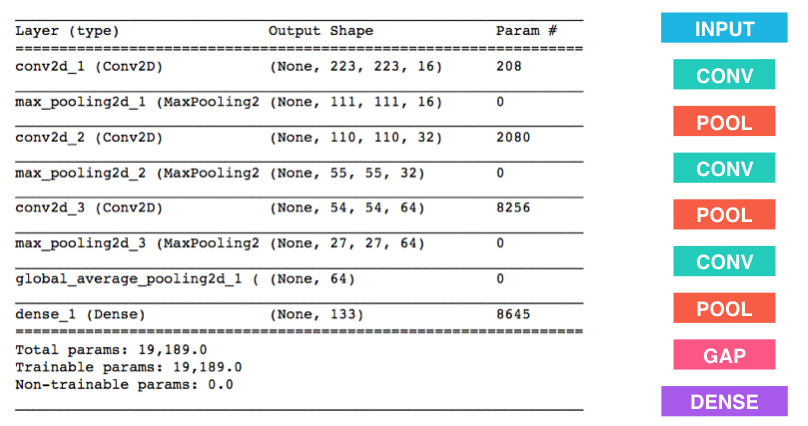
\includegraphics{images/sample_cnn.png}
\caption{Sample CNN}
\end{figure}

\textbf{Question 4:} Outline the steps you took to get to your final CNN
architecture and your reasoning at each step. If you chose to use the
hinted architecture above, describe why you think that CNN architecture
should work well for the image classification task.

\textbf{Answer:}

    \begin{Verbatim}[commandchars=\\\{\}]
{\color{incolor}In [{\color{incolor}14}]:} \PY{k+kn}{from} \PY{n+nn}{keras}\PY{n+nn}{.}\PY{n+nn}{layers} \PY{k}{import} \PY{n}{Conv2D}\PY{p}{,} \PY{n}{MaxPooling2D}\PY{p}{,} \PY{n}{GlobalAveragePooling2D}
         \PY{k+kn}{from} \PY{n+nn}{keras}\PY{n+nn}{.}\PY{n+nn}{layers} \PY{k}{import} \PY{n}{Dropout}\PY{p}{,} \PY{n}{Flatten}\PY{p}{,} \PY{n}{Dense}
         \PY{k+kn}{from} \PY{n+nn}{keras}\PY{n+nn}{.}\PY{n+nn}{models} \PY{k}{import} \PY{n}{Sequential}
         
         \PY{n}{model} \PY{o}{=} \PY{n}{Sequential}\PY{p}{(}\PY{p}{)}
         
         \PY{c+c1}{\PYZsh{}\PYZsh{}\PYZsh{} TODO: Define your architecture.}
         \PY{n}{model}\PY{o}{.}\PY{n}{add}\PY{p}{(}\PY{n}{Conv2D}\PY{p}{(}\PY{n}{filters}\PY{o}{=}\PY{l+m+mi}{16}\PY{p}{,} \PY{n}{kernel\PYZus{}size}\PY{o}{=}\PY{l+m+mi}{2}\PY{p}{,} \PY{n}{padding}\PY{o}{=}\PY{l+s+s1}{\PYZsq{}}\PY{l+s+s1}{same}\PY{l+s+s1}{\PYZsq{}}\PY{p}{,} \PY{n}{activation}\PY{o}{=}\PY{l+s+s1}{\PYZsq{}}\PY{l+s+s1}{relu}\PY{l+s+s1}{\PYZsq{}}\PY{p}{,}\PY{n}{input\PYZus{}shape}\PY{o}{=}\PY{p}{(}\PY{l+m+mi}{224}\PY{p}{,} \PY{l+m+mi}{224}\PY{p}{,} \PY{l+m+mi}{3}\PY{p}{)}\PY{p}{)}\PY{p}{)}
         \PY{n}{model}\PY{o}{.}\PY{n}{add}\PY{p}{(}\PY{n}{MaxPooling2D}\PY{p}{(}\PY{n}{pool\PYZus{}size}\PY{o}{=}\PY{l+m+mi}{2}\PY{p}{)}\PY{p}{)}
         \PY{n}{model}\PY{o}{.}\PY{n}{add}\PY{p}{(}\PY{n}{Conv2D}\PY{p}{(}\PY{n}{filters}\PY{o}{=}\PY{l+m+mi}{16}\PY{p}{,} \PY{n}{kernel\PYZus{}size}\PY{o}{=}\PY{l+m+mi}{2}\PY{p}{,} \PY{n}{activation}\PY{o}{=}\PY{l+s+s1}{\PYZsq{}}\PY{l+s+s1}{softplus}\PY{l+s+s1}{\PYZsq{}}\PY{p}{)}\PY{p}{)}
         \PY{n}{model}\PY{o}{.}\PY{n}{add}\PY{p}{(}\PY{n}{MaxPooling2D}\PY{p}{(}\PY{n}{pool\PYZus{}size}\PY{o}{=}\PY{l+m+mi}{2}\PY{p}{)}\PY{p}{)}
         \PY{n}{model}\PY{o}{.}\PY{n}{add}\PY{p}{(}\PY{n}{Conv2D}\PY{p}{(}\PY{n}{filters}\PY{o}{=}\PY{l+m+mi}{64}\PY{p}{,} \PY{n}{kernel\PYZus{}size}\PY{o}{=}\PY{l+m+mi}{2}\PY{p}{,} \PY{n}{padding}\PY{o}{=}\PY{l+s+s1}{\PYZsq{}}\PY{l+s+s1}{same}\PY{l+s+s1}{\PYZsq{}}\PY{p}{,} \PY{n}{activation}\PY{o}{=}\PY{l+s+s1}{\PYZsq{}}\PY{l+s+s1}{softplus}\PY{l+s+s1}{\PYZsq{}}\PY{p}{)}\PY{p}{)}
         \PY{n}{model}\PY{o}{.}\PY{n}{add}\PY{p}{(}\PY{n}{MaxPooling2D}\PY{p}{(}\PY{n}{pool\PYZus{}size}\PY{o}{=}\PY{l+m+mi}{2}\PY{p}{)}\PY{p}{)}
         \PY{n}{model}\PY{o}{.}\PY{n}{add}\PY{p}{(}\PY{n}{GlobalAveragePooling2D}\PY{p}{(}\PY{p}{)}\PY{p}{)}
         \PY{n}{model}\PY{o}{.}\PY{n}{add}\PY{p}{(}\PY{n}{Dense}\PY{p}{(}\PY{l+m+mi}{133}\PY{p}{,} \PY{n}{activation}\PY{o}{=}\PY{l+s+s1}{\PYZsq{}}\PY{l+s+s1}{softplus}\PY{l+s+s1}{\PYZsq{}}\PY{p}{)}\PY{p}{)}
         \PY{n}{model}\PY{o}{.}\PY{n}{summary}\PY{p}{(}\PY{p}{)}
\end{Verbatim}


    \begin{Verbatim}[commandchars=\\\{\}]
\_\_\_\_\_\_\_\_\_\_\_\_\_\_\_\_\_\_\_\_\_\_\_\_\_\_\_\_\_\_\_\_\_\_\_\_\_\_\_\_\_\_\_\_\_\_\_\_\_\_\_\_\_\_\_\_\_\_\_\_\_\_\_\_\_
Layer (type)                 Output Shape              Param \#   
=================================================================
conv2d\_1 (Conv2D)            (None, 224, 224, 16)      208       
\_\_\_\_\_\_\_\_\_\_\_\_\_\_\_\_\_\_\_\_\_\_\_\_\_\_\_\_\_\_\_\_\_\_\_\_\_\_\_\_\_\_\_\_\_\_\_\_\_\_\_\_\_\_\_\_\_\_\_\_\_\_\_\_\_
max\_pooling2d\_2 (MaxPooling2 (None, 112, 112, 16)      0         
\_\_\_\_\_\_\_\_\_\_\_\_\_\_\_\_\_\_\_\_\_\_\_\_\_\_\_\_\_\_\_\_\_\_\_\_\_\_\_\_\_\_\_\_\_\_\_\_\_\_\_\_\_\_\_\_\_\_\_\_\_\_\_\_\_
conv2d\_2 (Conv2D)            (None, 111, 111, 16)      1040      
\_\_\_\_\_\_\_\_\_\_\_\_\_\_\_\_\_\_\_\_\_\_\_\_\_\_\_\_\_\_\_\_\_\_\_\_\_\_\_\_\_\_\_\_\_\_\_\_\_\_\_\_\_\_\_\_\_\_\_\_\_\_\_\_\_
max\_pooling2d\_3 (MaxPooling2 (None, 55, 55, 16)        0         
\_\_\_\_\_\_\_\_\_\_\_\_\_\_\_\_\_\_\_\_\_\_\_\_\_\_\_\_\_\_\_\_\_\_\_\_\_\_\_\_\_\_\_\_\_\_\_\_\_\_\_\_\_\_\_\_\_\_\_\_\_\_\_\_\_
conv2d\_3 (Conv2D)            (None, 55, 55, 64)        4160      
\_\_\_\_\_\_\_\_\_\_\_\_\_\_\_\_\_\_\_\_\_\_\_\_\_\_\_\_\_\_\_\_\_\_\_\_\_\_\_\_\_\_\_\_\_\_\_\_\_\_\_\_\_\_\_\_\_\_\_\_\_\_\_\_\_
max\_pooling2d\_4 (MaxPooling2 (None, 27, 27, 64)        0         
\_\_\_\_\_\_\_\_\_\_\_\_\_\_\_\_\_\_\_\_\_\_\_\_\_\_\_\_\_\_\_\_\_\_\_\_\_\_\_\_\_\_\_\_\_\_\_\_\_\_\_\_\_\_\_\_\_\_\_\_\_\_\_\_\_
global\_average\_pooling2d\_1 ( (None, 64)                0         
\_\_\_\_\_\_\_\_\_\_\_\_\_\_\_\_\_\_\_\_\_\_\_\_\_\_\_\_\_\_\_\_\_\_\_\_\_\_\_\_\_\_\_\_\_\_\_\_\_\_\_\_\_\_\_\_\_\_\_\_\_\_\_\_\_
dense\_1 (Dense)              (None, 133)               8645      
=================================================================
Total params: 14,053
Trainable params: 14,053
Non-trainable params: 0
\_\_\_\_\_\_\_\_\_\_\_\_\_\_\_\_\_\_\_\_\_\_\_\_\_\_\_\_\_\_\_\_\_\_\_\_\_\_\_\_\_\_\_\_\_\_\_\_\_\_\_\_\_\_\_\_\_\_\_\_\_\_\_\_\_

    \end{Verbatim}

    \subsubsection{Compile the Model}\label{compile-the-model}

    \begin{Verbatim}[commandchars=\\\{\}]
{\color{incolor}In [{\color{incolor}15}]:} \PY{n}{model}\PY{o}{.}\PY{n}{compile}\PY{p}{(}\PY{n}{optimizer}\PY{o}{=}\PY{l+s+s1}{\PYZsq{}}\PY{l+s+s1}{adam}\PY{l+s+s1}{\PYZsq{}}\PY{p}{,} \PY{n}{loss}\PY{o}{=}\PY{l+s+s1}{\PYZsq{}}\PY{l+s+s1}{categorical\PYZus{}crossentropy}\PY{l+s+s1}{\PYZsq{}}\PY{p}{,} \PY{n}{metrics}\PY{o}{=}\PY{p}{[}\PY{l+s+s1}{\PYZsq{}}\PY{l+s+s1}{accuracy}\PY{l+s+s1}{\PYZsq{}}\PY{p}{]}\PY{p}{)}
\end{Verbatim}


    \begin{Verbatim}[commandchars=\\\{\}]
WARNING:tensorflow:From /home/samir/anaconda3/envs/py35/lib/python3.5/site-packages/keras/backend/tensorflow\_backend.py:2885: calling reduce\_sum (from tensorflow.python.ops.math\_ops) with keep\_dims is deprecated and will be removed in a future version.
Instructions for updating:
keep\_dims is deprecated, use keepdims instead

    \end{Verbatim}

    \subsubsection{(IMPLEMENTATION) Train the
Model}\label{implementation-train-the-model}

Train your model in the code cell below. Use model checkpointing to save
the model that attains the best validation loss.

You are welcome to
\href{https://blog.keras.io/building-powerful-image-classification-models-using-very-little-data.html}{augment
the training data}, but this is not a requirement.

    \begin{Verbatim}[commandchars=\\\{\}]
{\color{incolor}In [{\color{incolor}16}]:} \PY{k+kn}{from} \PY{n+nn}{keras}\PY{n+nn}{.}\PY{n+nn}{callbacks} \PY{k}{import} \PY{n}{ModelCheckpoint}  
         
         \PY{c+c1}{\PYZsh{}\PYZsh{}\PYZsh{} TODO: specify the number of epochs that you would like to use to train the model.}
         
         \PY{n}{epochs} \PY{o}{=} \PY{l+m+mi}{5}
         
         \PY{c+c1}{\PYZsh{}\PYZsh{}\PYZsh{} Do NOT modify the code below this line.}
         
         \PY{n}{checkpointer} \PY{o}{=} \PY{n}{ModelCheckpoint}\PY{p}{(}\PY{n}{filepath}\PY{o}{=}\PY{l+s+s1}{\PYZsq{}}\PY{l+s+s1}{saved\PYZus{}models/weights.best.from\PYZus{}scratch.hdf5}\PY{l+s+s1}{\PYZsq{}}\PY{p}{,} 
                                        \PY{n}{verbose}\PY{o}{=}\PY{l+m+mi}{1}\PY{p}{,} \PY{n}{save\PYZus{}best\PYZus{}only}\PY{o}{=}\PY{k+kc}{True}\PY{p}{)}
         
         \PY{n}{model}\PY{o}{.}\PY{n}{fit}\PY{p}{(}\PY{n}{train\PYZus{}tensors}\PY{p}{,} \PY{n}{train\PYZus{}targets}\PY{p}{,} 
                   \PY{n}{validation\PYZus{}data}\PY{o}{=}\PY{p}{(}\PY{n}{valid\PYZus{}tensors}\PY{p}{,} \PY{n}{valid\PYZus{}targets}\PY{p}{)}\PY{p}{,}
                   \PY{n}{epochs}\PY{o}{=}\PY{n}{epochs}\PY{p}{,} \PY{n}{batch\PYZus{}size}\PY{o}{=}\PY{l+m+mi}{20}\PY{p}{,} \PY{n}{callbacks}\PY{o}{=}\PY{p}{[}\PY{n}{checkpointer}\PY{p}{]}\PY{p}{,} \PY{n}{verbose}\PY{o}{=}\PY{l+m+mi}{1}\PY{p}{)}
\end{Verbatim}


    \begin{Verbatim}[commandchars=\\\{\}]
Train on 6680 samples, validate on 835 samples
Epoch 1/5
6660/6680 [============================>.] - ETA: 0s - loss: 4.8991 - acc: 0.0080Epoch 00001: val\_loss improved from inf to 4.87182, saving model to saved\_models/weights.best.from\_scratch.hdf5
6680/6680 [==============================] - 247s 37ms/step - loss: 4.8991 - acc: 0.0079 - val\_loss: 4.8718 - val\_acc: 0.0096
Epoch 2/5
6660/6680 [============================>.] - ETA: 0s - loss: 4.8766 - acc: 0.0092Epoch 00002: val\_loss improved from 4.87182 to 4.87053, saving model to saved\_models/weights.best.from\_scratch.hdf5
6680/6680 [==============================] - 229s 34ms/step - loss: 4.8767 - acc: 0.0091 - val\_loss: 4.8705 - val\_acc: 0.0108
Epoch 3/5
6660/6680 [============================>.] - ETA: 0s - loss: 4.8726 - acc: 0.0096Epoch 00003: val\_loss improved from 4.87053 to 4.86995, saving model to saved\_models/weights.best.from\_scratch.hdf5
6680/6680 [==============================] - 229s 34ms/step - loss: 4.8725 - acc: 0.0097 - val\_loss: 4.8699 - val\_acc: 0.0108
Epoch 4/5
6660/6680 [============================>.] - ETA: 0s - loss: 4.8707 - acc: 0.0092Epoch 00004: val\_loss improved from 4.86995 to 4.86925, saving model to saved\_models/weights.best.from\_scratch.hdf5
6680/6680 [==============================] - 233s 35ms/step - loss: 4.8707 - acc: 0.0091 - val\_loss: 4.8692 - val\_acc: 0.0108
Epoch 5/5
6660/6680 [============================>.] - ETA: 0s - loss: 4.8707 - acc: 0.0092Epoch 00005: val\_loss improved from 4.86925 to 4.86831, saving model to saved\_models/weights.best.from\_scratch.hdf5
6680/6680 [==============================] - 235s 35ms/step - loss: 4.8707 - acc: 0.0093 - val\_loss: 4.8683 - val\_acc: 0.0120

    \end{Verbatim}

\begin{Verbatim}[commandchars=\\\{\}]
{\color{outcolor}Out[{\color{outcolor}16}]:} <keras.callbacks.History at 0x7feac93cbf28>
\end{Verbatim}
            
    \subsubsection{Load the Model with the Best Validation
Loss}\label{load-the-model-with-the-best-validation-loss}

    \begin{Verbatim}[commandchars=\\\{\}]
{\color{incolor}In [{\color{incolor}17}]:} \PY{n}{model}\PY{o}{.}\PY{n}{load\PYZus{}weights}\PY{p}{(}\PY{l+s+s1}{\PYZsq{}}\PY{l+s+s1}{saved\PYZus{}models/weights.best.from\PYZus{}scratch.hdf5}\PY{l+s+s1}{\PYZsq{}}\PY{p}{)}
\end{Verbatim}


    \subsubsection{Test the Model}\label{test-the-model}

Try out your model on the test dataset of dog images. Ensure that your
test accuracy is greater than 1\%.

    \begin{Verbatim}[commandchars=\\\{\}]
{\color{incolor}In [{\color{incolor}18}]:} \PY{c+c1}{\PYZsh{} get index of predicted dog breed for each image in test set}
         \PY{n}{dog\PYZus{}breed\PYZus{}predictions} \PY{o}{=} \PY{p}{[}\PY{n}{np}\PY{o}{.}\PY{n}{argmax}\PY{p}{(}\PY{n}{model}\PY{o}{.}\PY{n}{predict}\PY{p}{(}\PY{n}{np}\PY{o}{.}\PY{n}{expand\PYZus{}dims}\PY{p}{(}\PY{n}{tensor}\PY{p}{,} \PY{n}{axis}\PY{o}{=}\PY{l+m+mi}{0}\PY{p}{)}\PY{p}{)}\PY{p}{)} \PY{k}{for} \PY{n}{tensor} \PY{o+ow}{in} \PY{n}{test\PYZus{}tensors}\PY{p}{]}
         
         \PY{c+c1}{\PYZsh{} report test accuracy}
         \PY{n}{test\PYZus{}accuracy} \PY{o}{=} \PY{l+m+mi}{100}\PY{o}{*}\PY{n}{np}\PY{o}{.}\PY{n}{sum}\PY{p}{(}\PY{n}{np}\PY{o}{.}\PY{n}{array}\PY{p}{(}\PY{n}{dog\PYZus{}breed\PYZus{}predictions}\PY{p}{)}\PY{o}{==}\PY{n}{np}\PY{o}{.}\PY{n}{argmax}\PY{p}{(}\PY{n}{test\PYZus{}targets}\PY{p}{,} \PY{n}{axis}\PY{o}{=}\PY{l+m+mi}{1}\PY{p}{)}\PY{p}{)}\PY{o}{/}\PY{n+nb}{len}\PY{p}{(}\PY{n}{dog\PYZus{}breed\PYZus{}predictions}\PY{p}{)}
         \PY{n+nb}{print}\PY{p}{(}\PY{l+s+s1}{\PYZsq{}}\PY{l+s+s1}{Test accuracy: }\PY{l+s+si}{\PYZpc{}.4f}\PY{l+s+si}{\PYZpc{}\PYZpc{}}\PY{l+s+s1}{\PYZsq{}} \PY{o}{\PYZpc{}} \PY{n}{test\PYZus{}accuracy}\PY{p}{)}
\end{Verbatim}


    \begin{Verbatim}[commandchars=\\\{\}]
Test accuracy: 1.0766\%

    \end{Verbatim}

    \begin{center}\rule{0.5\linewidth}{\linethickness}\end{center}

 \#\# Step 4: Use a CNN to Classify Dog Breeds

To reduce training time without sacrificing accuracy, we show you how to
train a CNN using transfer learning. In the following step, you will get
a chance to use transfer learning to train your own CNN.

\subsubsection{Obtain Bottleneck
Features}\label{obtain-bottleneck-features}

    \begin{Verbatim}[commandchars=\\\{\}]
{\color{incolor}In [{\color{incolor}19}]:} \PY{n}{bottleneck\PYZus{}features} \PY{o}{=} \PY{n}{np}\PY{o}{.}\PY{n}{load}\PY{p}{(}\PY{l+s+s1}{\PYZsq{}}\PY{l+s+s1}{bottleneck\PYZus{}features/DogVGG16Data.npz}\PY{l+s+s1}{\PYZsq{}}\PY{p}{)}
         \PY{n}{train\PYZus{}VGG16} \PY{o}{=} \PY{n}{bottleneck\PYZus{}features}\PY{p}{[}\PY{l+s+s1}{\PYZsq{}}\PY{l+s+s1}{train}\PY{l+s+s1}{\PYZsq{}}\PY{p}{]}
         \PY{n}{valid\PYZus{}VGG16} \PY{o}{=} \PY{n}{bottleneck\PYZus{}features}\PY{p}{[}\PY{l+s+s1}{\PYZsq{}}\PY{l+s+s1}{valid}\PY{l+s+s1}{\PYZsq{}}\PY{p}{]}
         \PY{n}{test\PYZus{}VGG16} \PY{o}{=} \PY{n}{bottleneck\PYZus{}features}\PY{p}{[}\PY{l+s+s1}{\PYZsq{}}\PY{l+s+s1}{test}\PY{l+s+s1}{\PYZsq{}}\PY{p}{]}
\end{Verbatim}


    \subsubsection{Model Architecture}\label{model-architecture}

The model uses the the pre-trained VGG-16 model as a fixed feature
extractor, where the last convolutional output of VGG-16 is fed as input
to our model. We only add a global average pooling layer and a fully
connected layer, where the latter contains one node for each dog
category and is equipped with a softmax.

    \begin{Verbatim}[commandchars=\\\{\}]
{\color{incolor}In [{\color{incolor}20}]:} \PY{n}{VGG16\PYZus{}model} \PY{o}{=} \PY{n}{Sequential}\PY{p}{(}\PY{p}{)}
         \PY{n}{VGG16\PYZus{}model}\PY{o}{.}\PY{n}{add}\PY{p}{(}\PY{n}{GlobalAveragePooling2D}\PY{p}{(}\PY{n}{input\PYZus{}shape}\PY{o}{=}\PY{n}{train\PYZus{}VGG16}\PY{o}{.}\PY{n}{shape}\PY{p}{[}\PY{l+m+mi}{1}\PY{p}{:}\PY{p}{]}\PY{p}{)}\PY{p}{)}
         \PY{n}{VGG16\PYZus{}model}\PY{o}{.}\PY{n}{add}\PY{p}{(}\PY{n}{Dense}\PY{p}{(}\PY{l+m+mi}{133}\PY{p}{,} \PY{n}{activation}\PY{o}{=}\PY{l+s+s1}{\PYZsq{}}\PY{l+s+s1}{softmax}\PY{l+s+s1}{\PYZsq{}}\PY{p}{)}\PY{p}{)}
         
         \PY{n}{VGG16\PYZus{}model}\PY{o}{.}\PY{n}{summary}\PY{p}{(}\PY{p}{)}
\end{Verbatim}


    \begin{Verbatim}[commandchars=\\\{\}]
\_\_\_\_\_\_\_\_\_\_\_\_\_\_\_\_\_\_\_\_\_\_\_\_\_\_\_\_\_\_\_\_\_\_\_\_\_\_\_\_\_\_\_\_\_\_\_\_\_\_\_\_\_\_\_\_\_\_\_\_\_\_\_\_\_
Layer (type)                 Output Shape              Param \#   
=================================================================
global\_average\_pooling2d\_2 ( (None, 512)               0         
\_\_\_\_\_\_\_\_\_\_\_\_\_\_\_\_\_\_\_\_\_\_\_\_\_\_\_\_\_\_\_\_\_\_\_\_\_\_\_\_\_\_\_\_\_\_\_\_\_\_\_\_\_\_\_\_\_\_\_\_\_\_\_\_\_
dense\_2 (Dense)              (None, 133)               68229     
=================================================================
Total params: 68,229
Trainable params: 68,229
Non-trainable params: 0
\_\_\_\_\_\_\_\_\_\_\_\_\_\_\_\_\_\_\_\_\_\_\_\_\_\_\_\_\_\_\_\_\_\_\_\_\_\_\_\_\_\_\_\_\_\_\_\_\_\_\_\_\_\_\_\_\_\_\_\_\_\_\_\_\_

    \end{Verbatim}

    \subsubsection{Compile the Model}\label{compile-the-model}

    \begin{Verbatim}[commandchars=\\\{\}]
{\color{incolor}In [{\color{incolor}21}]:} \PY{n}{VGG16\PYZus{}model}\PY{o}{.}\PY{n}{compile}\PY{p}{(}\PY{n}{loss}\PY{o}{=}\PY{l+s+s1}{\PYZsq{}}\PY{l+s+s1}{categorical\PYZus{}crossentropy}\PY{l+s+s1}{\PYZsq{}}\PY{p}{,} \PY{n}{optimizer}\PY{o}{=}\PY{l+s+s1}{\PYZsq{}}\PY{l+s+s1}{adam}\PY{l+s+s1}{\PYZsq{}}\PY{p}{,} \PY{n}{metrics}\PY{o}{=}\PY{p}{[}\PY{l+s+s1}{\PYZsq{}}\PY{l+s+s1}{accuracy}\PY{l+s+s1}{\PYZsq{}}\PY{p}{]}\PY{p}{)}
\end{Verbatim}


    \subsubsection{Train the Model}\label{train-the-model}

    \begin{Verbatim}[commandchars=\\\{\}]
{\color{incolor}In [{\color{incolor}22}]:} \PY{n}{checkpointer} \PY{o}{=} \PY{n}{ModelCheckpoint}\PY{p}{(}\PY{n}{filepath}\PY{o}{=}\PY{l+s+s1}{\PYZsq{}}\PY{l+s+s1}{saved\PYZus{}models/weights.best.VGG16.hdf5}\PY{l+s+s1}{\PYZsq{}}\PY{p}{,} 
                                        \PY{n}{verbose}\PY{o}{=}\PY{l+m+mi}{1}\PY{p}{,} \PY{n}{save\PYZus{}best\PYZus{}only}\PY{o}{=}\PY{k+kc}{True}\PY{p}{)}
         
         \PY{n}{VGG16\PYZus{}model}\PY{o}{.}\PY{n}{fit}\PY{p}{(}\PY{n}{train\PYZus{}VGG16}\PY{p}{,} \PY{n}{train\PYZus{}targets}\PY{p}{,} 
                   \PY{n}{validation\PYZus{}data}\PY{o}{=}\PY{p}{(}\PY{n}{valid\PYZus{}VGG16}\PY{p}{,} \PY{n}{valid\PYZus{}targets}\PY{p}{)}\PY{p}{,}
                   \PY{n}{epochs}\PY{o}{=}\PY{l+m+mi}{20}\PY{p}{,} \PY{n}{batch\PYZus{}size}\PY{o}{=}\PY{l+m+mi}{20}\PY{p}{,} \PY{n}{callbacks}\PY{o}{=}\PY{p}{[}\PY{n}{checkpointer}\PY{p}{]}\PY{p}{,} \PY{n}{verbose}\PY{o}{=}\PY{l+m+mi}{1}\PY{p}{)}
\end{Verbatim}


    \begin{Verbatim}[commandchars=\\\{\}]
Train on 6680 samples, validate on 835 samples
Epoch 1/20
6660/6680 [============================>.] - ETA: 0s - loss: 10.6689 - acc: 0.1850Epoch 00001: val\_loss improved from inf to 8.29594, saving model to saved\_models/weights.best.VGG16.hdf5
6680/6680 [==============================] - 2s 370us/step - loss: 10.6537 - acc: 0.1856 - val\_loss: 8.2959 - val\_acc: 0.3198
Epoch 2/20
6620/6680 [============================>.] - ETA: 0s - loss: 7.4761 - acc: 0.4230Epoch 00002: val\_loss improved from 8.29594 to 7.68167, saving model to saved\_models/weights.best.VGG16.hdf5
6680/6680 [==============================] - 2s 235us/step - loss: 7.4767 - acc: 0.4232 - val\_loss: 7.6817 - val\_acc: 0.3832
Epoch 3/20
6500/6680 [============================>.] - ETA: 0s - loss: 6.5807 - acc: 0.5194Epoch 00003: val\_loss improved from 7.68167 to 7.13097, saving model to saved\_models/weights.best.VGG16.hdf5
6680/6680 [==============================] - 2s 232us/step - loss: 6.5976 - acc: 0.5183 - val\_loss: 7.1310 - val\_acc: 0.4311
Epoch 4/20
6460/6680 [============================>.] - ETA: 0s - loss: 6.3144 - acc: 0.5615Epoch 00004: val\_loss improved from 7.13097 to 6.96501, saving model to saved\_models/weights.best.VGG16.hdf5
6680/6680 [==============================] - 2s 234us/step - loss: 6.3272 - acc: 0.5605 - val\_loss: 6.9650 - val\_acc: 0.4599
Epoch 5/20
6500/6680 [============================>.] - ETA: 0s - loss: 6.2291 - acc: 0.5849Epoch 00005: val\_loss did not improve
6680/6680 [==============================] - 2s 242us/step - loss: 6.2161 - acc: 0.5855 - val\_loss: 6.9812 - val\_acc: 0.4479
Epoch 6/20
6420/6680 [===========================>..] - ETA: 0s - loss: 6.2030 - acc: 0.6040Epoch 00006: val\_loss improved from 6.96501 to 6.84790, saving model to saved\_models/weights.best.VGG16.hdf5
6680/6680 [==============================] - 2s 233us/step - loss: 6.1520 - acc: 0.6069 - val\_loss: 6.8479 - val\_acc: 0.4743
Epoch 7/20
6460/6680 [============================>.] - ETA: 0s - loss: 6.1017 - acc: 0.6119Epoch 00007: val\_loss improved from 6.84790 to 6.84284, saving model to saved\_models/weights.best.VGG16.hdf5
6680/6680 [==============================] - 2s 233us/step - loss: 6.1308 - acc: 0.6102 - val\_loss: 6.8428 - val\_acc: 0.4874
Epoch 8/20
6640/6680 [============================>.] - ETA: 0s - loss: 6.1031 - acc: 0.6155Epoch 00008: val\_loss did not improve
6680/6680 [==============================] - 2s 234us/step - loss: 6.1172 - acc: 0.6147 - val\_loss: 6.8603 - val\_acc: 0.4838
Epoch 9/20
6660/6680 [============================>.] - ETA: 0s - loss: 6.1163 - acc: 0.6155Epoch 00009: val\_loss did not improve
6680/6680 [==============================] - 2s 232us/step - loss: 6.1125 - acc: 0.6157 - val\_loss: 6.9495 - val\_acc: 0.4719
Epoch 10/20
6540/6680 [============================>.] - ETA: 0s - loss: 6.1296 - acc: 0.6102Epoch 00010: val\_loss did not improve
6680/6680 [==============================] - 2s 231us/step - loss: 6.1336 - acc: 0.6097 - val\_loss: 7.0605 - val\_acc: 0.4491
Epoch 11/20
6420/6680 [===========================>..] - ETA: 0s - loss: 6.2372 - acc: 0.5844Epoch 00011: val\_loss did not improve
6680/6680 [==============================] - 2s 231us/step - loss: 6.2495 - acc: 0.5829 - val\_loss: 7.1813 - val\_acc: 0.4563
Epoch 12/20
6540/6680 [============================>.] - ETA: 0s - loss: 6.2231 - acc: 0.5841Epoch 00012: val\_loss did not improve
6680/6680 [==============================] - 2s 228us/step - loss: 6.2375 - acc: 0.5831 - val\_loss: 7.1728 - val\_acc: 0.4515
Epoch 13/20
6480/6680 [============================>.] - ETA: 0s - loss: 6.1746 - acc: 0.6049Epoch 00013: val\_loss did not improve
6680/6680 [==============================] - 2s 230us/step - loss: 6.1624 - acc: 0.6055 - val\_loss: 6.9364 - val\_acc: 0.4874
Epoch 14/20
6480/6680 [============================>.] - ETA: 0s - loss: 6.0935 - acc: 0.6165Epoch 00014: val\_loss did not improve
6680/6680 [==============================] - 2s 232us/step - loss: 6.1144 - acc: 0.6148 - val\_loss: 7.0114 - val\_acc: 0.4874
Epoch 15/20
6560/6680 [============================>.] - ETA: 0s - loss: 6.1669 - acc: 0.6085Epoch 00015: val\_loss did not improve
6680/6680 [==============================] - 2s 234us/step - loss: 6.1556 - acc: 0.6091 - val\_loss: 6.8873 - val\_acc: 0.4934
Epoch 16/20
6440/6680 [===========================>..] - ETA: 0s - loss: 6.1357 - acc: 0.6123Epoch 00016: val\_loss did not improve
6680/6680 [==============================] - 2s 230us/step - loss: 6.1187 - acc: 0.6132 - val\_loss: 7.0110 - val\_acc: 0.4790
Epoch 17/20
6540/6680 [============================>.] - ETA: 0s - loss: 6.2104 - acc: 0.6011Epoch 00017: val\_loss did not improve
6680/6680 [==============================] - 2s 230us/step - loss: 6.1673 - acc: 0.6036 - val\_loss: 7.1094 - val\_acc: 0.4802
Epoch 18/20
6440/6680 [===========================>..] - ETA: 0s - loss: 6.1732 - acc: 0.6056Epoch 00018: val\_loss did not improve
6680/6680 [==============================] - 2s 231us/step - loss: 6.1460 - acc: 0.6066 - val\_loss: 7.0372 - val\_acc: 0.4826
Epoch 19/20
6600/6680 [============================>.] - ETA: 0s - loss: 6.1110 - acc: 0.6091Epoch 00019: val\_loss did not improve
6680/6680 [==============================] - 2s 233us/step - loss: 6.1464 - acc: 0.6070 - val\_loss: 7.0102 - val\_acc: 0.4898
Epoch 20/20
6480/6680 [============================>.] - ETA: 0s - loss: 6.1084 - acc: 0.6160Epoch 00020: val\_loss did not improve
6680/6680 [==============================] - 2s 232us/step - loss: 6.1090 - acc: 0.6162 - val\_loss: 6.9736 - val\_acc: 0.4814

    \end{Verbatim}

\begin{Verbatim}[commandchars=\\\{\}]
{\color{outcolor}Out[{\color{outcolor}22}]:} <keras.callbacks.History at 0x7fea971a00f0>
\end{Verbatim}
            
    \subsubsection{Load the Model with the Best Validation
Loss}\label{load-the-model-with-the-best-validation-loss}

    \begin{Verbatim}[commandchars=\\\{\}]
{\color{incolor}In [{\color{incolor}23}]:} \PY{n}{VGG16\PYZus{}model}\PY{o}{.}\PY{n}{load\PYZus{}weights}\PY{p}{(}\PY{l+s+s1}{\PYZsq{}}\PY{l+s+s1}{saved\PYZus{}models/weights.best.VGG16.hdf5}\PY{l+s+s1}{\PYZsq{}}\PY{p}{)}
\end{Verbatim}


    \subsubsection{Test the Model}\label{test-the-model}

Now, we can use the CNN to test how well it identifies breed within our
test dataset of dog images. We print the test accuracy below.

    \begin{Verbatim}[commandchars=\\\{\}]
{\color{incolor}In [{\color{incolor}24}]:} \PY{c+c1}{\PYZsh{} get index of predicted dog breed for each image in test set}
         \PY{n}{VGG16\PYZus{}predictions} \PY{o}{=} \PY{p}{[}\PY{n}{np}\PY{o}{.}\PY{n}{argmax}\PY{p}{(}\PY{n}{VGG16\PYZus{}model}\PY{o}{.}\PY{n}{predict}\PY{p}{(}\PY{n}{np}\PY{o}{.}\PY{n}{expand\PYZus{}dims}\PY{p}{(}\PY{n}{feature}\PY{p}{,} \PY{n}{axis}\PY{o}{=}\PY{l+m+mi}{0}\PY{p}{)}\PY{p}{)}\PY{p}{)} \PY{k}{for} \PY{n}{feature} \PY{o+ow}{in} \PY{n}{test\PYZus{}VGG16}\PY{p}{]}
         
         \PY{c+c1}{\PYZsh{} report test accuracy}
         \PY{n}{test\PYZus{}accuracy} \PY{o}{=} \PY{l+m+mi}{100}\PY{o}{*}\PY{n}{np}\PY{o}{.}\PY{n}{sum}\PY{p}{(}\PY{n}{np}\PY{o}{.}\PY{n}{array}\PY{p}{(}\PY{n}{VGG16\PYZus{}predictions}\PY{p}{)}\PY{o}{==}\PY{n}{np}\PY{o}{.}\PY{n}{argmax}\PY{p}{(}\PY{n}{test\PYZus{}targets}\PY{p}{,} \PY{n}{axis}\PY{o}{=}\PY{l+m+mi}{1}\PY{p}{)}\PY{p}{)}\PY{o}{/}\PY{n+nb}{len}\PY{p}{(}\PY{n}{VGG16\PYZus{}predictions}\PY{p}{)}
         \PY{n+nb}{print}\PY{p}{(}\PY{l+s+s1}{\PYZsq{}}\PY{l+s+s1}{Test accuracy: }\PY{l+s+si}{\PYZpc{}.4f}\PY{l+s+si}{\PYZpc{}\PYZpc{}}\PY{l+s+s1}{\PYZsq{}} \PY{o}{\PYZpc{}} \PY{n}{test\PYZus{}accuracy}\PY{p}{)}
\end{Verbatim}


    \begin{Verbatim}[commandchars=\\\{\}]
Test accuracy: 47.7273\%

    \end{Verbatim}

    \subsubsection{Predict Dog Breed with the
Model}\label{predict-dog-breed-with-the-model}

    \begin{Verbatim}[commandchars=\\\{\}]
{\color{incolor}In [{\color{incolor}25}]:} \PY{k+kn}{from} \PY{n+nn}{extract\PYZus{}bottleneck\PYZus{}features} \PY{k}{import} \PY{o}{*}
         
         \PY{k}{def} \PY{n+nf}{VGG16\PYZus{}predict\PYZus{}breed}\PY{p}{(}\PY{n}{img\PYZus{}path}\PY{p}{)}\PY{p}{:}
             \PY{c+c1}{\PYZsh{} extract bottleneck features}
             \PY{n}{bottleneck\PYZus{}feature} \PY{o}{=} \PY{n}{extract\PYZus{}VGG16}\PY{p}{(}\PY{n}{path\PYZus{}to\PYZus{}tensor}\PY{p}{(}\PY{n}{img\PYZus{}path}\PY{p}{)}\PY{p}{)}
             \PY{c+c1}{\PYZsh{} obtain predicted vector}
             \PY{n}{predicted\PYZus{}vector} \PY{o}{=} \PY{n}{VGG16\PYZus{}model}\PY{o}{.}\PY{n}{predict}\PY{p}{(}\PY{n}{bottleneck\PYZus{}feature}\PY{p}{)}
             \PY{c+c1}{\PYZsh{} return dog breed that is predicted by the model}
             \PY{k}{return} \PY{n}{dog\PYZus{}names}\PY{p}{[}\PY{n}{np}\PY{o}{.}\PY{n}{argmax}\PY{p}{(}\PY{n}{predicted\PYZus{}vector}\PY{p}{)}\PY{p}{]}
\end{Verbatim}


    \begin{center}\rule{0.5\linewidth}{\linethickness}\end{center}

 \#\# Step 5: Create a CNN to Classify Dog Breeds (using Transfer
Learning)

You will now use transfer learning to create a CNN that can identify dog
breed from images. Your CNN must attain at least 60\% accuracy on the
test set.

In Step 4, we used transfer learning to create a CNN using VGG-16
bottleneck features. In this section, you must use the bottleneck
features from a different pre-trained model. To make things easier for
you, we have pre-computed the features for all of the networks that are
currently available in Keras: -
\href{https://s3-us-west-1.amazonaws.com/udacity-aind/dog-project/DogVGG19Data.npz}{VGG-19}
bottleneck features -
\href{https://s3-us-west-1.amazonaws.com/udacity-aind/dog-project/DogResnet50Data.npz}{ResNet-50}
bottleneck features -
\href{https://s3-us-west-1.amazonaws.com/udacity-aind/dog-project/DogInceptionV3Data.npz}{Inception}
bottleneck features -
\href{https://s3-us-west-1.amazonaws.com/udacity-aind/dog-project/DogXceptionData.npz}{Xception}
bottleneck features

The files are encoded as such:

\begin{verbatim}
Dog{network}Data.npz
\end{verbatim}

where \texttt{\{network\}}, in the above filename, can be one of
\texttt{VGG19}, \texttt{Resnet50}, \texttt{InceptionV3}, or
\texttt{Xception}. Pick one of the above architectures, download the
corresponding bottleneck features, and store the downloaded file in the
\texttt{bottleneck\_features/} folder in the repository.

\subsubsection{(IMPLEMENTATION) Obtain Bottleneck
Features}\label{implementation-obtain-bottleneck-features}

In the code block below, extract the bottleneck features corresponding
to the train, test, and validation sets by running the following:

\begin{verbatim}
bottleneck_features = np.load('bottleneck_features/Dog{network}Data.npz')
train_{network} = bottleneck_features['train']
valid_{network} = bottleneck_features['valid']
test_{network} = bottleneck_features['test']
\end{verbatim}

    \begin{Verbatim}[commandchars=\\\{\}]
{\color{incolor}In [{\color{incolor}26}]:} \PY{c+c1}{\PYZsh{}\PYZsh{}\PYZsh{} TODO: Obtain bottleneck features from another pre\PYZhy{}trained CNN.}
         
         \PY{n}{bottleneck\PYZus{}features} \PY{o}{=} \PY{n}{np}\PY{o}{.}\PY{n}{load}\PY{p}{(}\PY{l+s+s1}{\PYZsq{}}\PY{l+s+s1}{bottleneck\PYZus{}features/DogResnet50Data.npz}\PY{l+s+s1}{\PYZsq{}}\PY{p}{)}
         \PY{n}{train\PYZus{}Resnet50} \PY{o}{=} \PY{n}{bottleneck\PYZus{}features}\PY{p}{[}\PY{l+s+s1}{\PYZsq{}}\PY{l+s+s1}{train}\PY{l+s+s1}{\PYZsq{}}\PY{p}{]}
         \PY{n}{valid\PYZus{}Resnet50} \PY{o}{=} \PY{n}{bottleneck\PYZus{}features}\PY{p}{[}\PY{l+s+s1}{\PYZsq{}}\PY{l+s+s1}{valid}\PY{l+s+s1}{\PYZsq{}}\PY{p}{]}
         \PY{n}{test\PYZus{}Resnet50} \PY{o}{=} \PY{n}{bottleneck\PYZus{}features}\PY{p}{[}\PY{l+s+s1}{\PYZsq{}}\PY{l+s+s1}{test}\PY{l+s+s1}{\PYZsq{}}\PY{p}{]}
\end{Verbatim}


    \subsubsection{(IMPLEMENTATION) Model
Architecture}\label{implementation-model-architecture}

Create a CNN to classify dog breed. At the end of your code cell block,
summarize the layers of your model by executing the line:

\begin{verbatim}
    <your model's name>.summary()
\end{verbatim}

\textbf{Question 5:} Outline the steps you took to get to your final CNN
architecture and your reasoning at each step. Describe why you think the
architecture is suitable for the current problem.

\textbf{Answer:}

    \begin{Verbatim}[commandchars=\\\{\}]
{\color{incolor}In [{\color{incolor}27}]:} \PY{c+c1}{\PYZsh{}\PYZsh{}\PYZsh{} TODO: Define your architecture.}
         
         \PY{n}{Resnet50\PYZus{}model} \PY{o}{=} \PY{n}{Sequential}\PY{p}{(}\PY{p}{)}
         \PY{n}{Resnet50\PYZus{}model}\PY{o}{.}\PY{n}{add}\PY{p}{(}\PY{n}{GlobalAveragePooling2D}\PY{p}{(}\PY{n}{input\PYZus{}shape}\PY{o}{=}\PY{n}{train\PYZus{}Resnet50}\PY{o}{.}\PY{n}{shape}\PY{p}{[}\PY{l+m+mi}{1}\PY{p}{:}\PY{p}{]}\PY{p}{)}\PY{p}{)}
         \PY{n}{Resnet50\PYZus{}model}\PY{o}{.}\PY{n}{add}\PY{p}{(}\PY{n}{Dropout}\PY{p}{(}\PY{l+m+mf}{0.25}\PY{p}{)}\PY{p}{)}
         \PY{n}{Resnet50\PYZus{}model}\PY{o}{.}\PY{n}{add}\PY{p}{(}\PY{n}{Dense}\PY{p}{(}\PY{l+m+mi}{133}\PY{p}{,} \PY{n}{activation}\PY{o}{=}\PY{l+s+s1}{\PYZsq{}}\PY{l+s+s1}{softmax}\PY{l+s+s1}{\PYZsq{}}\PY{p}{)}\PY{p}{)}
         
         \PY{n}{Resnet50\PYZus{}model}\PY{o}{.}\PY{n}{summary}\PY{p}{(}\PY{p}{)}
\end{Verbatim}


    \begin{Verbatim}[commandchars=\\\{\}]
\_\_\_\_\_\_\_\_\_\_\_\_\_\_\_\_\_\_\_\_\_\_\_\_\_\_\_\_\_\_\_\_\_\_\_\_\_\_\_\_\_\_\_\_\_\_\_\_\_\_\_\_\_\_\_\_\_\_\_\_\_\_\_\_\_
Layer (type)                 Output Shape              Param \#   
=================================================================
global\_average\_pooling2d\_3 ( (None, 2048)              0         
\_\_\_\_\_\_\_\_\_\_\_\_\_\_\_\_\_\_\_\_\_\_\_\_\_\_\_\_\_\_\_\_\_\_\_\_\_\_\_\_\_\_\_\_\_\_\_\_\_\_\_\_\_\_\_\_\_\_\_\_\_\_\_\_\_
dropout\_1 (Dropout)          (None, 2048)              0         
\_\_\_\_\_\_\_\_\_\_\_\_\_\_\_\_\_\_\_\_\_\_\_\_\_\_\_\_\_\_\_\_\_\_\_\_\_\_\_\_\_\_\_\_\_\_\_\_\_\_\_\_\_\_\_\_\_\_\_\_\_\_\_\_\_
dense\_3 (Dense)              (None, 133)               272517    
=================================================================
Total params: 272,517
Trainable params: 272,517
Non-trainable params: 0
\_\_\_\_\_\_\_\_\_\_\_\_\_\_\_\_\_\_\_\_\_\_\_\_\_\_\_\_\_\_\_\_\_\_\_\_\_\_\_\_\_\_\_\_\_\_\_\_\_\_\_\_\_\_\_\_\_\_\_\_\_\_\_\_\_

    \end{Verbatim}

    \subsubsection{(IMPLEMENTATION) Compile the
Model}\label{implementation-compile-the-model}

    \begin{Verbatim}[commandchars=\\\{\}]
{\color{incolor}In [{\color{incolor}28}]:} \PY{c+c1}{\PYZsh{}\PYZsh{}\PYZsh{} TODO: Compile the model.}
         \PY{n}{Resnet50\PYZus{}model}\PY{o}{.}\PY{n}{compile}\PY{p}{(}\PY{n}{loss}\PY{o}{=}\PY{l+s+s1}{\PYZsq{}}\PY{l+s+s1}{categorical\PYZus{}crossentropy}\PY{l+s+s1}{\PYZsq{}}\PY{p}{,} \PY{n}{optimizer}\PY{o}{=}\PY{l+s+s1}{\PYZsq{}}\PY{l+s+s1}{adam}\PY{l+s+s1}{\PYZsq{}}\PY{p}{,} \PY{n}{metrics}\PY{o}{=}\PY{p}{[}\PY{l+s+s1}{\PYZsq{}}\PY{l+s+s1}{accuracy}\PY{l+s+s1}{\PYZsq{}}\PY{p}{]}\PY{p}{)}
\end{Verbatim}


    \subsubsection{(IMPLEMENTATION) Train the
Model}\label{implementation-train-the-model}

Train your model in the code cell below. Use model checkpointing to save
the model that attains the best validation loss.

You are welcome to
\href{https://blog.keras.io/building-powerful-image-classification-models-using-very-little-data.html}{augment
the training data}, but this is not a requirement.

    \begin{Verbatim}[commandchars=\\\{\}]
{\color{incolor}In [{\color{incolor}29}]:} \PY{c+c1}{\PYZsh{}\PYZsh{}\PYZsh{} TODO: Train the model.}
         
         \PY{k+kn}{from} \PY{n+nn}{keras}\PY{n+nn}{.}\PY{n+nn}{callbacks} \PY{k}{import} \PY{n}{ModelCheckpoint}  
         \PY{k+kn}{from} \PY{n+nn}{keras} \PY{k}{import} \PY{n}{callbacks}
         \PY{n}{checkpointer} \PY{o}{=} \PY{n}{ModelCheckpoint}\PY{p}{(}\PY{n}{filepath}\PY{o}{=}\PY{l+s+s1}{\PYZsq{}}\PY{l+s+s1}{saved\PYZus{}models/weights.best.Resnet50.hdf5}\PY{l+s+s1}{\PYZsq{}}\PY{p}{,} 
                                        \PY{n}{verbose}\PY{o}{=}\PY{l+m+mi}{1}\PY{p}{,} \PY{n}{save\PYZus{}best\PYZus{}only}\PY{o}{=}\PY{k+kc}{True}\PY{p}{)}
         
         \PY{n}{Resnet50\PYZus{}model}\PY{o}{.}\PY{n}{fit}\PY{p}{(}\PY{n}{train\PYZus{}Resnet50}\PY{p}{,} \PY{n}{train\PYZus{}targets}\PY{p}{,} 
                   \PY{n}{validation\PYZus{}data}\PY{o}{=}\PY{p}{(}\PY{n}{valid\PYZus{}Resnet50}\PY{p}{,} \PY{n}{valid\PYZus{}targets}\PY{p}{)}\PY{p}{,}
                   \PY{n}{epochs}\PY{o}{=}\PY{l+m+mi}{20} \PY{p}{,} \PY{n}{batch\PYZus{}size}\PY{o}{=}\PY{l+m+mi}{50}\PY{p}{,} \PY{n}{callbacks}\PY{o}{=}\PY{p}{[}\PY{n}{checkpointer}\PY{p}{]}\PY{p}{,} \PY{n}{verbose}\PY{o}{=}\PY{l+m+mi}{1}\PY{p}{)}
\end{Verbatim}


    \begin{Verbatim}[commandchars=\\\{\}]
Train on 6680 samples, validate on 835 samples
Epoch 1/20
6600/6680 [============================>.] - ETA: 0s - loss: 2.2669 - acc: 0.4850Epoch 00001: val\_loss improved from inf to 0.99203, saving model to saved\_models/weights.best.Resnet50.hdf5
6680/6680 [==============================] - 2s 327us/step - loss: 2.2516 - acc: 0.4883 - val\_loss: 0.9920 - val\_acc: 0.7257
Epoch 2/20
6500/6680 [============================>.] - ETA: 0s - loss: 0.6286 - acc: 0.8332Epoch 00002: val\_loss improved from 0.99203 to 0.72023, saving model to saved\_models/weights.best.Resnet50.hdf5
6680/6680 [==============================] - 1s 212us/step - loss: 0.6245 - acc: 0.8343 - val\_loss: 0.7202 - val\_acc: 0.8036
Epoch 3/20
6650/6680 [============================>.] - ETA: 0s - loss: 0.3782 - acc: 0.9020Epoch 00003: val\_loss improved from 0.72023 to 0.66112, saving model to saved\_models/weights.best.Resnet50.hdf5
6680/6680 [==============================] - 1s 213us/step - loss: 0.3781 - acc: 0.9019 - val\_loss: 0.6611 - val\_acc: 0.8036
Epoch 4/20
6550/6680 [============================>.] - ETA: 0s - loss: 0.2448 - acc: 0.9455Epoch 00004: val\_loss improved from 0.66112 to 0.60090, saving model to saved\_models/weights.best.Resnet50.hdf5
6680/6680 [==============================] - 1s 215us/step - loss: 0.2447 - acc: 0.9452 - val\_loss: 0.6009 - val\_acc: 0.8180
Epoch 5/20
6400/6680 [===========================>..] - ETA: 0s - loss: 0.1761 - acc: 0.9652Epoch 00005: val\_loss improved from 0.60090 to 0.58682, saving model to saved\_models/weights.best.Resnet50.hdf5
6680/6680 [==============================] - 1s 220us/step - loss: 0.1779 - acc: 0.9647 - val\_loss: 0.5868 - val\_acc: 0.8192
Epoch 6/20
6600/6680 [============================>.] - ETA: 0s - loss: 0.1297 - acc: 0.9779Epoch 00006: val\_loss improved from 0.58682 to 0.56416, saving model to saved\_models/weights.best.Resnet50.hdf5
6680/6680 [==============================] - 1s 219us/step - loss: 0.1295 - acc: 0.9778 - val\_loss: 0.5642 - val\_acc: 0.8311
Epoch 7/20
6550/6680 [============================>.] - ETA: 0s - loss: 0.0993 - acc: 0.9873Epoch 00007: val\_loss did not improve
6680/6680 [==============================] - 1s 214us/step - loss: 0.0999 - acc: 0.9870 - val\_loss: 0.5805 - val\_acc: 0.8180
Epoch 8/20
6400/6680 [===========================>..] - ETA: 0s - loss: 0.0798 - acc: 0.9911Epoch 00008: val\_loss improved from 0.56416 to 0.55391, saving model to saved\_models/weights.best.Resnet50.hdf5
6680/6680 [==============================] - 1s 212us/step - loss: 0.0806 - acc: 0.9904 - val\_loss: 0.5539 - val\_acc: 0.8335
Epoch 9/20
6550/6680 [============================>.] - ETA: 0s - loss: 0.0661 - acc: 0.9936Epoch 00009: val\_loss improved from 0.55391 to 0.54896, saving model to saved\_models/weights.best.Resnet50.hdf5
6680/6680 [==============================] - 1s 215us/step - loss: 0.0665 - acc: 0.9934 - val\_loss: 0.5490 - val\_acc: 0.8311
Epoch 10/20
6600/6680 [============================>.] - ETA: 0s - loss: 0.0601 - acc: 0.9944Epoch 00010: val\_loss did not improve
6680/6680 [==============================] - 1s 211us/step - loss: 0.0598 - acc: 0.9945 - val\_loss: 0.5613 - val\_acc: 0.8216
Epoch 11/20
6550/6680 [============================>.] - ETA: 0s - loss: 0.0504 - acc: 0.9944Epoch 00011: val\_loss did not improve
6680/6680 [==============================] - 1s 212us/step - loss: 0.0507 - acc: 0.9943 - val\_loss: 0.5819 - val\_acc: 0.8383
Epoch 12/20
6450/6680 [===========================>..] - ETA: 0s - loss: 0.0448 - acc: 0.9961Epoch 00012: val\_loss did not improve
6680/6680 [==============================] - 1s 211us/step - loss: 0.0455 - acc: 0.9958 - val\_loss: 0.5552 - val\_acc: 0.8323
Epoch 13/20
6600/6680 [============================>.] - ETA: 0s - loss: 0.0377 - acc: 0.9973Epoch 00013: val\_loss did not improve
6680/6680 [==============================] - 1s 212us/step - loss: 0.0375 - acc: 0.9973 - val\_loss: 0.5498 - val\_acc: 0.8479
Epoch 14/20
6500/6680 [============================>.] - ETA: 0s - loss: 0.0352 - acc: 0.9972Epoch 00014: val\_loss improved from 0.54896 to 0.54137, saving model to saved\_models/weights.best.Resnet50.hdf5
6680/6680 [==============================] - 1s 213us/step - loss: 0.0349 - acc: 0.9973 - val\_loss: 0.5414 - val\_acc: 0.8443
Epoch 15/20
6600/6680 [============================>.] - ETA: 0s - loss: 0.0323 - acc: 0.9965Epoch 00015: val\_loss did not improve
6680/6680 [==============================] - 1s 212us/step - loss: 0.0322 - acc: 0.9966 - val\_loss: 0.5581 - val\_acc: 0.8491
Epoch 16/20
6650/6680 [============================>.] - ETA: 0s - loss: 0.0281 - acc: 0.9973Epoch 00016: val\_loss did not improve
6680/6680 [==============================] - 1s 215us/step - loss: 0.0282 - acc: 0.9973 - val\_loss: 0.5650 - val\_acc: 0.8275
Epoch 17/20
6650/6680 [============================>.] - ETA: 0s - loss: 0.0263 - acc: 0.9977Epoch 00017: val\_loss did not improve
6680/6680 [==============================] - 1s 214us/step - loss: 0.0262 - acc: 0.9978 - val\_loss: 0.5789 - val\_acc: 0.8347
Epoch 18/20
6550/6680 [============================>.] - ETA: 0s - loss: 0.0240 - acc: 0.9973Epoch 00018: val\_loss did not improve
6680/6680 [==============================] - 1s 213us/step - loss: 0.0243 - acc: 0.9970 - val\_loss: 0.5574 - val\_acc: 0.8347
Epoch 19/20
6450/6680 [===========================>..] - ETA: 0s - loss: 0.0217 - acc: 0.9983Epoch 00019: val\_loss did not improve
6680/6680 [==============================] - 1s 213us/step - loss: 0.0216 - acc: 0.9984 - val\_loss: 0.5618 - val\_acc: 0.8407
Epoch 20/20
6600/6680 [============================>.] - ETA: 0s - loss: 0.0227 - acc: 0.9971Epoch 00020: val\_loss did not improve
6680/6680 [==============================] - 1s 212us/step - loss: 0.0226 - acc: 0.9972 - val\_loss: 0.5686 - val\_acc: 0.8419

    \end{Verbatim}

\begin{Verbatim}[commandchars=\\\{\}]
{\color{outcolor}Out[{\color{outcolor}29}]:} <keras.callbacks.History at 0x7fea733cfc18>
\end{Verbatim}
            
    \subsubsection{(IMPLEMENTATION) Load the Model with the Best Validation
Loss}\label{implementation-load-the-model-with-the-best-validation-loss}

    \begin{Verbatim}[commandchars=\\\{\}]
{\color{incolor}In [{\color{incolor}30}]:} \PY{c+c1}{\PYZsh{}\PYZsh{}\PYZsh{} TODO: Load the model weights with the best validation loss.}
         \PY{n}{Resnet50\PYZus{}model}\PY{o}{.}\PY{n}{load\PYZus{}weights}\PY{p}{(}\PY{l+s+s1}{\PYZsq{}}\PY{l+s+s1}{saved\PYZus{}models/weights.best.Resnet50.hdf5}\PY{l+s+s1}{\PYZsq{}}\PY{p}{)}
\end{Verbatim}


    \subsubsection{(IMPLEMENTATION) Test the
Model}\label{implementation-test-the-model}

Try out your model on the test dataset of dog images. Ensure that your
test accuracy is greater than 60\%.

    \begin{Verbatim}[commandchars=\\\{\}]
{\color{incolor}In [{\color{incolor}31}]:} \PY{c+c1}{\PYZsh{}\PYZsh{}\PYZsh{} TODO: Calculate classification accuracy on the test dataset.}
         
         \PY{n}{dog\PYZus{}breed\PYZus{}predictions} \PY{o}{=} \PY{p}{[}\PY{n}{np}\PY{o}{.}\PY{n}{argmax}\PY{p}{(}\PY{n}{Resnet50\PYZus{}model}\PY{o}{.}\PY{n}{predict}\PY{p}{(}\PY{n}{np}\PY{o}{.}\PY{n}{expand\PYZus{}dims}\PY{p}{(}\PY{n}{tensor}\PY{p}{,} \PY{n}{axis}\PY{o}{=}\PY{l+m+mi}{0}\PY{p}{)}\PY{p}{)}\PY{p}{)} \PY{k}{for} \PY{n}{tensor} \PY{o+ow}{in} \PY{n}{test\PYZus{}Resnet50}\PY{p}{]}
         
         \PY{n}{test\PYZus{}accuracy} \PY{o}{=} \PY{l+m+mi}{100}\PY{o}{*}\PY{n}{np}\PY{o}{.}\PY{n}{sum}\PY{p}{(}\PY{n}{np}\PY{o}{.}\PY{n}{array}\PY{p}{(}\PY{n}{dog\PYZus{}breed\PYZus{}predictions}\PY{p}{)}\PY{o}{==}\PY{n}{np}\PY{o}{.}\PY{n}{argmax}\PY{p}{(}\PY{n}{test\PYZus{}targets}\PY{p}{,} \PY{n}{axis}\PY{o}{=}\PY{l+m+mi}{1}\PY{p}{)}\PY{p}{)}\PY{o}{/}\PY{n+nb}{len}\PY{p}{(}\PY{n}{dog\PYZus{}breed\PYZus{}predictions}\PY{p}{)}
         \PY{n+nb}{print}\PY{p}{(}\PY{l+s+s1}{\PYZsq{}}\PY{l+s+s1}{Test accuracy: }\PY{l+s+si}{\PYZpc{}.4f}\PY{l+s+si}{\PYZpc{}\PYZpc{}}\PY{l+s+s1}{\PYZsq{}} \PY{o}{\PYZpc{}} \PY{n}{test\PYZus{}accuracy}\PY{p}{)}
\end{Verbatim}


    \begin{Verbatim}[commandchars=\\\{\}]
Test accuracy: 83.3732\%

    \end{Verbatim}

    \subsubsection{(IMPLEMENTATION) Predict Dog Breed with the
Model}\label{implementation-predict-dog-breed-with-the-model}

Write a function that takes an image path as input and returns the dog
breed (\texttt{Affenpinscher}, \texttt{Afghan\_hound}, etc) that is
predicted by your model.

Similar to the analogous function in Step 5, your function should have
three steps: 1. Extract the bottleneck features corresponding to the
chosen CNN model. 2. Supply the bottleneck features as input to the
model to return the predicted vector. Note that the argmax of this
prediction vector gives the index of the predicted dog breed. 3. Use the
\texttt{dog\_names} array defined in Step 0 of this notebook to return
the corresponding breed.

The functions to extract the bottleneck features can be found in
\texttt{extract\_bottleneck\_features.py}, and they have been imported
in an earlier code cell. To obtain the bottleneck features corresponding
to your chosen CNN architecture, you need to use the function

\begin{verbatim}
extract_{network}
\end{verbatim}

where \texttt{\{network\}}, in the above filename, should be one of
\texttt{VGG19}, \texttt{Resnet50}, \texttt{InceptionV3}, or
\texttt{Xception}.

    \begin{Verbatim}[commandchars=\\\{\}]
{\color{incolor}In [{\color{incolor}32}]:} \PY{c+c1}{\PYZsh{}\PYZsh{}\PYZsh{} TODO: Write a function that takes a path to an image as input}
         \PY{c+c1}{\PYZsh{}\PYZsh{}\PYZsh{} and returns the dog breed that is predicted by the model.}
         
         \PY{k+kn}{from} \PY{n+nn}{extract\PYZus{}bottleneck\PYZus{}features} \PY{k}{import} \PY{o}{*}
         
         \PY{k}{def} \PY{n+nf}{Resnet50\PYZus{}predict\PYZus{}breed}\PY{p}{(}\PY{n}{img\PYZus{}path}\PY{p}{)}\PY{p}{:}
             \PY{n}{bottleneck\PYZus{}feature} \PY{o}{=} \PY{n}{extract\PYZus{}Resnet50}\PY{p}{(}\PY{n}{path\PYZus{}to\PYZus{}tensor}\PY{p}{(}\PY{n}{img\PYZus{}path}\PY{p}{)}\PY{p}{)}
             \PY{n}{predicted\PYZus{}vector} \PY{o}{=} \PY{n}{Resnet50\PYZus{}model}\PY{o}{.}\PY{n}{predict}\PY{p}{(}\PY{n}{bottleneck\PYZus{}feature}\PY{p}{)}
             \PY{k}{return} \PY{n}{dog\PYZus{}names}\PY{p}{[}\PY{n}{np}\PY{o}{.}\PY{n}{argmax}\PY{p}{(}\PY{n}{predicted\PYZus{}vector}\PY{p}{)}\PY{p}{]}
\end{Verbatim}


    \begin{center}\rule{0.5\linewidth}{\linethickness}\end{center}

 \#\# Step 6: Write your Algorithm

Write an algorithm that accepts a file path to an image and first
determines whether the image contains a human, dog, or neither. Then, -
if a \textbf{dog} is detected in the image, return the predicted breed.
- if a \textbf{human} is detected in the image, return the resembling
dog breed. - if \textbf{neither} is detected in the image, provide
output that indicates an error.

You are welcome to write your own functions for detecting humans and
dogs in images, but feel free to use the \texttt{face\_detector} and
\texttt{dog\_detector} functions developed above. You are
\textbf{required} to use your CNN from Step 5 to predict dog breed.

Some sample output for our algorithm is provided below, but feel free to
design your own user experience!

\begin{figure}
\centering
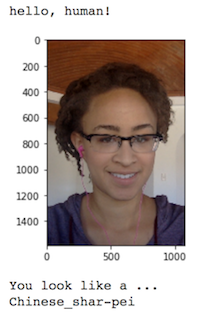
\includegraphics{images/sample_human_output.png}
\caption{Sample Human Output}
\end{figure}

\subsubsection{(IMPLEMENTATION) Write your
Algorithm}\label{implementation-write-your-algorithm}

    \begin{Verbatim}[commandchars=\\\{\}]
{\color{incolor}In [{\color{incolor}33}]:} \PY{c+c1}{\PYZsh{}\PYZsh{}\PYZsh{} TODO: Write your algorithm.}
         \PY{c+c1}{\PYZsh{}\PYZsh{}\PYZsh{} Feel free to use as many code cells as needed.}
         
         \PY{k+kn}{from} \PY{n+nn}{keras}\PY{n+nn}{.}\PY{n+nn}{preprocessing} \PY{k}{import} \PY{n}{image}                  
         \PY{k+kn}{from} \PY{n+nn}{os} \PY{k}{import} \PY{o}{*}
         \PY{k+kn}{import} \PY{n+nn}{random}
         
         \PY{k}{def} \PY{n+nf}{show\PYZus{}image}\PY{p}{(}\PY{n}{path}\PY{p}{)}\PY{p}{:}
             \PY{n}{img} \PY{o}{=} \PY{n}{image}\PY{o}{.}\PY{n}{load\PYZus{}img}\PY{p}{(}\PY{n}{path}\PY{p}{)}
             \PY{n}{img} \PY{o}{=} \PY{n}{image}\PY{o}{.}\PY{n}{img\PYZus{}to\PYZus{}array}\PY{p}{(}\PY{n}{img}\PY{p}{)}
             \PY{n}{plt}\PY{o}{.}\PY{n}{imshow}\PY{p}{(}\PY{n}{img}\PY{o}{/}\PY{l+m+mi}{255}\PY{p}{)}
             \PY{n}{plt}\PY{o}{.}\PY{n}{show}\PY{p}{(}\PY{p}{)}
             
         \PY{k}{def} \PY{n+nf}{predicts\PYZus{}dog\PYZus{}breed}\PY{p}{(}\PY{n}{path}\PY{p}{)}\PY{p}{:}
             \PY{n}{show\PYZus{}image}\PY{p}{(}\PY{n}{path}\PY{p}{)}
             \PY{n}{img} \PY{o}{=} \PY{n}{cv2}\PY{o}{.}\PY{n}{imread}\PY{p}{(}\PY{n}{path}\PY{p}{,}\PY{o}{\PYZhy{}}\PY{l+m+mi}{1}\PY{p}{)}
             \PY{n}{img\PYZus{}resize} \PY{o}{=} \PY{n}{cv2}\PY{o}{.}\PY{n}{resize}\PY{p}{(}\PY{n}{img}\PY{p}{,}\PY{p}{(}\PY{l+m+mi}{224}\PY{p}{,}\PY{l+m+mi}{224}\PY{p}{)}\PY{p}{)}
             \PY{n}{cv2}\PY{o}{.}\PY{n}{imwrite}\PY{p}{(}\PY{l+s+s1}{\PYZsq{}}\PY{l+s+s1}{test.jpg}\PY{l+s+s1}{\PYZsq{}}\PY{p}{,}\PY{n}{img\PYZus{}resize}\PY{p}{)}
             
             \PY{k}{if} \PY{p}{(}\PY{n}{face\PYZus{}detector}\PY{p}{(}\PY{n}{path}\PY{p}{)}\PY{p}{)}\PY{p}{:} \PY{c+c1}{\PYZsh{}if it\PYZsq{}s a human}
                 \PY{n+nb}{print} \PY{p}{(}\PY{l+s+s2}{\PYZdq{}}\PY{l+s+s2}{It}\PY{l+s+s2}{\PYZsq{}}\PY{l+s+s2}{s human: }\PY{l+s+s2}{\PYZdq{}}\PY{p}{)}
                 \PY{n}{dog\PYZus{}breed} \PY{o}{=} \PY{n}{Resnet50\PYZus{}predict\PYZus{}breed}\PY{p}{(}\PY{l+s+s1}{\PYZsq{}}\PY{l+s+s1}{test.jpg}\PY{l+s+s1}{\PYZsq{}}\PY{p}{)}
                 \PY{n+nb}{print} \PY{p}{(}\PY{l+s+s2}{\PYZdq{}}\PY{l+s+s2}{ look like }\PY{l+s+s2}{\PYZdq{}}\PY{p}{,} \PY{n}{dog\PYZus{}breed} \PY{p}{)}
             
             \PY{k}{elif} \PY{p}{(}\PY{n}{dog\PYZus{}detector}\PY{p}{(}\PY{l+s+s1}{\PYZsq{}}\PY{l+s+s1}{test.jpg}\PY{l+s+s1}{\PYZsq{}}\PY{p}{)}\PY{o}{==}\PY{l+m+mi}{1}\PY{p}{)}\PY{p}{:} \PY{c+c1}{\PYZsh{}if it\PYZsq{}s a dog}
                 \PY{n+nb}{print}\PY{p}{(}\PY{l+s+s2}{\PYZdq{}}\PY{l+s+s2}{It}\PY{l+s+s2}{\PYZsq{}}\PY{l+s+s2}{s dog }\PY{l+s+s2}{\PYZdq{}}\PY{p}{)}
                 \PY{n}{dog\PYZus{}breed} \PY{o}{=} \PY{n}{Resnet50\PYZus{}predict\PYZus{}breed}\PY{p}{(}\PY{l+s+s1}{\PYZsq{}}\PY{l+s+s1}{test.jpg}\PY{l+s+s1}{\PYZsq{}}\PY{p}{)}
                 \PY{n+nb}{print} \PY{p}{(}\PY{l+s+s2}{\PYZdq{}}\PY{l+s+s2}{Dog type is  :}\PY{l+s+s2}{\PYZdq{}}\PY{p}{,} \PY{n}{dog\PYZus{}breed} \PY{p}{)}
         
             \PY{k}{else}\PY{p}{:} \PY{c+c1}{\PYZsh{}for something else}
                 \PY{n+nb}{print} \PY{p}{(}\PY{l+s+s2}{\PYZdq{}}\PY{l+s+s2}{Not Dog nor Human }\PY{l+s+s2}{\PYZdq{}}\PY{p}{)}
             
             \PY{n}{os}\PY{o}{.}\PY{n}{remove}\PY{p}{(}\PY{l+s+s1}{\PYZsq{}}\PY{l+s+s1}{test.jpg}\PY{l+s+s1}{\PYZsq{}}\PY{p}{)}
             
\end{Verbatim}


    \begin{center}\rule{0.5\linewidth}{\linethickness}\end{center}

 \#\# Step 7: Test Your Algorithm

In this section, you will take your new algorithm for a spin! What kind
of dog does the algorithm think that \textbf{you} look like? If you have
a dog, does it predict your dog's breed accurately? If you have a cat,
does it mistakenly think that your cat is a dog?

\subsubsection{(IMPLEMENTATION) Test Your Algorithm on Sample
Images!}\label{implementation-test-your-algorithm-on-sample-images}

Test your algorithm at least six images on your computer. Feel free to
use any images you like. Use at least two human and two dog images.

\textbf{Question 6:} Is the output better than you expected :) ? Or
worse :( ? Provide at least three possible points of improvement for
your algorithm.

\textbf{Answer:}

    \begin{Verbatim}[commandchars=\\\{\}]
{\color{incolor}In [{\color{incolor}34}]:} \PY{c+c1}{\PYZsh{}\PYZsh{} TODO: Execute your algorithm from Step 6 on}
         \PY{c+c1}{\PYZsh{}\PYZsh{} at least 6 images on your computer.}
         \PY{c+c1}{\PYZsh{}\PYZsh{} Feel free to use as many code cells as needed.}
         
         \PY{n}{data} \PY{o}{=} \PY{n}{np}\PY{o}{.}\PY{n}{array}\PY{p}{(}\PY{n}{glob}\PY{p}{(}\PY{l+s+s2}{\PYZdq{}}\PY{l+s+s2}{images/*}\PY{l+s+s2}{\PYZdq{}}\PY{p}{)}\PY{p}{)}
         \PY{k}{for} \PY{n}{i} \PY{o+ow}{in} \PY{n}{data}\PY{p}{:}
             \PY{n}{predicts\PYZus{}dog\PYZus{}breed}\PY{p}{(}\PY{n}{i}\PY{p}{)}
\end{Verbatim}


    \begin{center}
    \adjustimage{max size={0.9\linewidth}{0.9\paperheight}}{output_65_0.png}
    \end{center}
    { \hspace*{\fill} \\}
    
    \begin{Verbatim}[commandchars=\\\{\}]
It's dog 
Dog type is  : Boykin\_spaniel

    \end{Verbatim}

    \begin{center}
    \adjustimage{max size={0.9\linewidth}{0.9\paperheight}}{output_65_2.png}
    \end{center}
    { \hspace*{\fill} \\}
    
    \begin{Verbatim}[commandchars=\\\{\}]
It's dog 
Dog type is  : Labrador\_retriever

    \end{Verbatim}

    \begin{center}
    \adjustimage{max size={0.9\linewidth}{0.9\paperheight}}{output_65_4.png}
    \end{center}
    { \hspace*{\fill} \\}
    
    \begin{Verbatim}[commandchars=\\\{\}]
It's dog 
Dog type is  : Welsh\_springer\_spaniel

    \end{Verbatim}

    \begin{center}
    \adjustimage{max size={0.9\linewidth}{0.9\paperheight}}{output_65_6.png}
    \end{center}
    { \hspace*{\fill} \\}
    
    \begin{Verbatim}[commandchars=\\\{\}]
Not Dog nor Human 

    \end{Verbatim}

    \begin{center}
    \adjustimage{max size={0.9\linewidth}{0.9\paperheight}}{output_65_8.png}
    \end{center}
    { \hspace*{\fill} \\}
    
    \begin{Verbatim}[commandchars=\\\{\}]
It's human: 
 look like  Norwegian\_lundehund

    \end{Verbatim}

    \begin{center}
    \adjustimage{max size={0.9\linewidth}{0.9\paperheight}}{output_65_10.png}
    \end{center}
    { \hspace*{\fill} \\}
    
    \begin{Verbatim}[commandchars=\\\{\}]
It's dog 
Dog type is  : Labrador\_retriever

    \end{Verbatim}

    \begin{center}
    \adjustimage{max size={0.9\linewidth}{0.9\paperheight}}{output_65_12.png}
    \end{center}
    { \hspace*{\fill} \\}
    
    \begin{Verbatim}[commandchars=\\\{\}]
It's dog 
Dog type is  : Brittany

    \end{Verbatim}

    \begin{center}
    \adjustimage{max size={0.9\linewidth}{0.9\paperheight}}{output_65_14.png}
    \end{center}
    { \hspace*{\fill} \\}
    
    \begin{Verbatim}[commandchars=\\\{\}]
It's dog 
Dog type is  : Curly-coated\_retriever

    \end{Verbatim}

    \begin{center}
    \adjustimage{max size={0.9\linewidth}{0.9\paperheight}}{output_65_16.png}
    \end{center}
    { \hspace*{\fill} \\}
    
    \begin{Verbatim}[commandchars=\\\{\}]
It's dog 
Dog type is  : Labrador\_retriever

    \end{Verbatim}


    % Add a bibliography block to the postdoc
    
    
    
    \end{document}
